\documentclass{article}
\usepackage{amsfonts}
\usepackage{graphicx}
\usepackage[margin=1in]{geometry}
\usepackage{bm}
\usepackage{amsmath}
\usepackage{authblk}
\usepackage{caption}
\usepackage{hyperref}
\usepackage{float}
\usepackage[parfill]{parskip}
%\renewcommand{\familydefault}{\sfdefault}

\title{cILR: Taxonomic Enrichment Analysis with Isometric Log-Ratios}
\author[1,2]{Quang P. Nguyen}
\author[1,2]{Anne G. Hoen}
\author[1]{H. Robert Frost}
\affil[1]{Department of Biomedical Data Science, Geisel School of Medicine at Dartmouth College, Hanover, NH, USA}
\affil[2]{Department of Epidemiology, Geisel School of Medicine at Dartmouth College, Hanover, NH, USA}
\date{}                     %% if you don't need a date to appear
\setcounter{Maxaffil}{0}
\renewcommand\Affilfont{\itshape\small}

\begin{document}
\maketitle
\captionsetup[figure]{labelfont={bf},name={Figure},labelsep=period, margin=1cm}

\begin{abstract}
    \noindent Research in human associated microbiomes primarily involve the analysis of taxonomic count tables generated via high-throughput sequencing. It is difficult to apply statistical tools as the data is high-dimensional, sparse, and strictly compositional. An approachable way to alleviate high-dimensionality and sparsity is to aggregate variables into pre-defined sets. Set-based analysis is ubiquitous in the genomics literature, and have demonstrable impact in improving interpretability and power of downstream analysis. Current practice in the microbiome field, however, performs aggregation by summing the abundance of respective taxa. This approach prevents comparison across sets of different sizes, does not preserve inter-sample distances, and amplifies protocol bias. Unfortunately, there is a lack of interest in developing more sophisticated set-based analysis methods specific to microbiome data. Here, we attempt to fill this gap with a new sample-level taxon set enrichment method based on the isometric log ratio transformation and the competitive null hypothesis commonly used in the enrichment analysis literature. Our approach, titled competitive isometric log ratio (cILR), generates sample-specific enrichment scores as the scaled log ratio of the subcomposition defined by taxa within a set and the subcomposition defined by its complement. We provide sample-level significance testing by estimating an empirical null distribution of our test statistic with valid p-values. Herein we demonstrate under both real data applications and simulations that cILR controls for type I error even under high sparsity and high inter-taxa correlation scenarios, while additionally providing informative scores that can be inputs to downstream differential abundance and predictive tasks with good performance. These results demonstrate how our approach can enable researchers to generate meaningful aggregation scores for sets of taxa. 
\end{abstract}

\section*{Background}  
The microbiome is the collection of microorganisms (bacteria, protozoa, archaea, fungi, and viruses) which co-exist with their human host. Previous research has shown that changes in the composition of the microbiome are associated with important health outcomes such as inflammatory bowel disease \cite{proctor2019}, type II diabetes \cite{sharma2019}, and obesity \cite{aoun2020}. To understand the central role of the microbiome in human health, researchers have relied on high-throughput sequencing methods, either by targeting a specific representative gene (i.e. amplicon sequencing) or by profiling all the genomic content of the sample (i.e. whole-genome shotgun sequencing) \cite{cho2012}. Processing raw sequencing data using a variety of bioinformatic pipelines \cite{callahan2016,truong2015} yields taxonomic abundance tables that can be used in downstream statistical analyses to identify associations between an outcome/exposure and identified taxa.  

However, there exists unique challenges in the analysis of these data tables \cite{li2019,li2015}. First, like other sequencing-based datasets, microbiome count data is often high dimensional, where the number of detected taxa far exceeds the number of samples usually present. For predictive tasks, microbiome-specific penalized regression approaches have been developed to address this issue \cite{shi2016}, allowing for simultaneous model fitting and variable selection. For differential abundance tasks, researchers often utilize multiple hypothesis correction methods \cite{sankaran2014,benjamini1995} or omnibus tests \cite{chen2018} to address hypothesis testing burden. 

Second, the number of reads obtained is constrained by the sequencing instrument at an arbitrary limit, and applied inconsistently across samples, resulting in a different number of total read counts per sample. Many normalization methods \cite{weiss2017} have been proposed to address these issues, including cross-applying methods from the gene expression literature \cite{mcmurdie2014}. However, these methods rely on assumptions specific to the original bulk RNA-seq data sets such as the presence of housekeeping genes with consistent expression levels \cite{love2014}, which might not be not true in the context of microbiome relative abundance data \cite{quinn2019,quinn2018b}. As such, microbiome data is strictly compositional \cite{gloor2017}, which means that the abundance of any taxa can only be interpreted relative to another. Consequently, log-ratio transformations from the compositional data literature are often utilized \cite{aitchison1999}. 

Third, the data is highly zero-inflated, where there is a high number of both structural zeros (truly missing due to biological reasons) and sampling zeroes (due to limits of detection of the sequencing experiment). Researchers often dealt with these issues by imputing zero cells with a pseudocount \cite{kurtz2015}, or applying zero-inflated models \cite{chen2018, kaul2017}. Newer methods developed recently have focused on understanding the different types of zeros in the data, providing more sophisticated heuristics around when pseudocounts can be utilized \cite{kaul2017a}.   

Even though the aforementioned problems are challenging, a very approachable method to address some of them is through set-based analysis, also termed gene set testing in the genomics literature \cite{khatri2012, goeman2007}. Aggregated sets can be less sparse than their constituent elements, and testing on a smaller number of variables can reduce the multiple testing burden, thereby increasing power and reproducibility. Through the usage of functionally informative sets defined apriori based on historical experiments (for example MSigDB \cite{subramanian2005}, and Gene Ontology \cite{ashburner2000}), gene set analyses also allows for more informative interpretations. There exists a diverse set of available methods developed to perform such analyses. More traditional set testing methods utilize the hypergeometric test to test for the overrepresentation of significant p-values for a set of interest \cite{goeman2007}. Unfortunately, these approaches are sensitive to the differential expression test and their generated p-values. The most widely used gene-set analysis method, GSEA \cite{subramanian2005}, instead uses a random-walk-like statistic through a ranking of genes based on a measure of association or effect size. Both of these methods generate enrichment scores and significance testing at the population level, incorporating information from all samples. Conversely, methods such as GSVA \cite{hanzelmann2013} and VAM \cite{frost2020a}, generate enrichment scores at the sample and is more akin to a transformation. This strategy allows for the flexible incorporation of different statistical techniques downstream, such as predictive models, as well as for visualization purposes in ordination plots.  

In microbiome research, even though no explicit enrichment analysis is performed, standard practice often involves aggregating taxa to higher Linnean classification levels such as genus, family, or phylum by simple summation of abundances \cite{mclaren2019}. Even though this allows for a reduction in the number of overall taxa (from thousands to only hundreds), there still exist three disadvantages: first, inter-sample distances are not preserved before and after aggregation \cite{egozcue2005}, second, it doesn't allow for enrichment testing and comparison across sets of different sizes, and third, increase bias when taxa within the set have different efficiencies in how they are measured through sequencing \cite{mclaren2019}. As such, there is a need for microbiome researchers to adopt set enrichment methods to perform a more robust analysis that allows for enrichment testing of functionally relevant sets of microbes. Unfortunately, there is a lack of interest in extending existing methods to be more specific to microbiome relative abundance data. Some software suites, such as \emph{MicrobiomeAnalyst}, do provide researchers tools to perform enrichment testing with curated taxa sets \cite{chong2020}. However, the approach used in \emph{MicrobiomeAnalyst} is an overrepresentation analysis and therefore similarly sensitive to the method of differential abundance used. 

Here, we developed a novel method that allows for generating enrichment scores at the sample level similar to GSVA \cite{hanzelmann2013} and VAM \cite{frost2020a}. We leverage the conception of the $Q_1$ competitive hypothesis presented in Tian et al. \cite{tian2005}, which compares the expression of genes within the gene set against the rest of the genes. The competitive hypothesis is particularly useful in compositional data analysis, as it naturally assesses enrichment as a ratio between two sets of variables. We incorporated this insight with the isometric log-ratio transformation \cite{egozcue2003}, which allows for a multiplicative aggregation method that addresses the downsides of the naive summation-based method presented above \cite{mclaren2019, silverman2017}. The resulting method, titled competitive isometric log-ratio (cILR), is therefore unsupervised and can generate sample-specific enrichment scores with a well-defined null hypothesis that allows for significance testing. These scores can then act as inputs to differential abundance and predictive modeling tasks downstream. 

In the following sections, we provide the formulation of cILR and discuss some statistical properties. Then, we illustrate significance testing at the sample level using cILR and demonstrating type I error and power under different simulation scenarios and real data applications. Then we assessed the informativeness of cILR generated scores, and evaluated how it performs as part of downstream analyses, specifically predictive models and differential abundance analysis. We compare the performance of cILR in these respective tasks against standard microbiome data analysis practices, as well as existing GSVA \cite{hanzelmann2013} and ssGSEA \cite{barbie2009}, which are equivalent single sample enrichment analysis methods in the genomics literature. An R package implementation of this approach can be found on Github (\href{www.github.com/qpmnguyen/teaR}{qpmnguyen/teaR}).

\section*{Materials and Methods} \label{Methods}
\subsection*{Competitive Isometric Log-ratio (cILR)}
The cILR method generates sample-specific enrichment scores for microbial sets using the isometric log-ratio transformation \cite{egozcue2003}. Details on the computational implementation of cILR can be found in the supplemental materials. The cILR method takes two inputs:  
\begin{itemize}
    \item $\mathbf{X}$: $n$ by $p$ matrix of positive counts for $p$ taxa and $n$ samples measured through either targeted sequencing (such as of the 16S rRNA gene) or whole genome shotgun sequencing. Usually $\mathbf{X}$ is generated from standard taxonomic profiling pipelines such as DADA2 \cite{callahan2016} for 16S rRNA sequencing, or MetaPhlAn2 \cite{truong2015} for whole genome shotgun sequencing. 
    \item $\mathbf{A}$: $p$ by $m$ indicator matrix annotating the membership of each taxon $p$ to $m$ sets of interest. These sets can be Linnean taxonomic classifications annotated using databases such as SILVA \cite{quast2013}, or those based on more functionally driven categories such as tropism or ecosystem roles ($A_{i,j} = 1$ indicates that microbe $i$ belongs to set $j$). 
\end{itemize}
The cILR method generates one output:  
\begin{itemize} 
    \item $\mathbf{E}$: $n$ by $m$ matrix indicating the enrichment score of $m$ pre-defined sets identified in $\mathbf{A}$ across $n$ samples. 
\end{itemize}
The procedure is as follows:  
\begin{enumerate}
    \item \textbf{Compute the cILR statistic}: Let $\mathbf{M}$ be a $n$ by $m$ matrix of cILR scores. Let $\mathbf{M}_{i,k}$ be cILR scores for set $k$ of sample $i$:   
    \begin{equation}\label{main_eq}
        \mathbf{M}_{i,k} = \sqrt{\frac{\sum_k A_{ik}(p - \sum_k A_{ik})}{p}} \ln \left( \frac{g(\mathbf{X}_{i,j}|\mathbf{A}_{j,k} = 1)}{g(\mathbf{X}_{i,j}|\mathbf{A}_{j,k} \neq 1))} \right)
    \end{equation}
    where $g(.)$ is the geometric mean. This represents the ratio of the geometric mean of the relative abundance of taxa assigned to set $k$ and remainder taxa. 
    \item \textbf{Estimate the empirical null distribution} Enrichment scores represent the test statistic for the $Q_1$ null hypothesis $H_o$ that relative abundances in $\mathbf{X}$ of members of set $k$ are not enriched compared to those not in set $k$. Since the distribution of cILR under the null vary depending on data characteristics (Figure \ref{fig:kurt_gof}), an empirical null distribution will be estimated from data.
    \begin{itemize}
        \item \textbf{Compute the cILR statistic on permuted and un-permuted $\mathbf{X}$}.  Let $\mathbf{X}_{perm}$ be the column permuted relative abundance matrix, and $\mathbf{M}_{perm}$ be the corresponding cILR scores generated from $\mathbf{X}_{perm}$. Similarly, we have $\mathbf{M}_{unperm}$ be cILR scores generated from $\mathbf{X}$.
        \item \textbf{Estimate correlation-adjusted empirical distribution for each set}. For each set, a fit a parametric distribution to both $\mathbf{M}_{perm}$ and $\mathbf{M}_{unperm}$. The location measure estimated from $\mathbf{M}_{perm}$ and the spread measure estimated from $\mathbf{M}_{unperm}$ will be combined as the correlation-adjusted empirical null distribution $\mathbf{P}_{emp}$ for each set. Two available options are the normal distribution and the mixture normal distribution. For the normal distribution, parameters were estimated using the method of maximum likelihood implemented in the \emph{fitdistr} package \cite{delignette-muller2015}. For the mixture normal distribution, parameters were estimated using an expectation-maximization algorithm implemented in the \emph{mixtools} package \cite{benaglia2009}. 
    \end{itemize}
    \item \textbf{Calculate finalized cILR scores with respect to the empirical null}. Enrichment scores $\mathbf{E}_{i,k}$ are calculated as the cumulative distribution function (CDF) values or z-scores with respect to $\mathbf{P}_{emp}$ distribution. Valid p-values can be calculated by subtracting $\mathbf{E}$ from 1. 
\end{enumerate}



\subsection*{Properties of cILR}
\subsubsection*{cILR and the Isometric Log Ratio Transformation}
The cILR statistic is a special instance of the isometric log-ratio transformation (ILR) \cite{egozcue2003}. The standard ILR is a transformation method to address the negative correlation bias inherent in compositional data by providing an isometry between the $D$-dimensional simplex $\mathbb{S}^D$ and coordinates in the $D-1$ real space $\mathbb{R}^{D-1}$ \cite{egozcue2003,washburne2017}. This is accomplished by projecting the composition onto a chosen orthonormal basis in $\mathbb{R}$, which can be defined by a sequential binary partition (SBP) of the variables (e.g. a rooted phylogenetic tree). The ILR transformed variables are the coordinates of nodes within an SBP tree of the variables. Without loss of generalizability, in a given SBP with node $i$ splitting variables between sets $R$ and $S$, we have the ILR coordinate $x^{*}_{i}$ as: 
\begin{equation}\label{ilr_standard}
    x^{*}_i = \sqrt{\frac{rs}{r+s}} \log\left(\frac{g(X_{j|j \in R})}{g(X_{j|j \in S})}\right)
\end{equation}
where $r$ and $s$ are the cardinalities of sets $R$ and $S$ respectively, $g(z)$ is the geometric mean, and $X_{j}$ are values of the original predictors with indexes defined by membership in $R$ and $S$. The ILR confer many important benefits. First, ILR coordinates exist in real space, whereby common statistical methods can be used. Second, ILR aggregated variables preserve inter-sample distances before and after aggregation \cite{egozcue2005}. Third, ILR variables are not constrained to sum to 0 as that of the centered log-ratio transformation, resulting in a covariance matrix that is not singular \cite{egozcue2003}. 

The usage of the ILR statistic is not uncommon in the microbiome literature. They are usually termed ``compositional balances", and have been leveraged in many recent approaches in variable transformation \cite{washburne2017,silverman2017,morton2017}. The cILR formulation \eqref{main_eq} is a special case of \eqref{ilr_standard} defined on a node that splits the taxa into two disjoint sets, one representing the set of interest, the other representing the remaining taxa. As such, the cILR transformation inherits the properties of the ILR as a log-ratio method applicable to compositional data sets. However, unlike the ILR and its variants \cite{silverman2017, morton2017, washburne2017}, the axes defined by each cILR set are not orthogonal (since the balances are mutually exclusive between sets and do not belong in the same SBP). Hence, a correlation can exist between cILR aggregated variables.  

\subsubsection*{Statistical Properties of cILR}
We can perform significance testing on the cILR statistic which corresponds to the null hypothesis that the center of the subcomposition defined by the set is equal to the center of the subcomposition defined by the complement of the set. This is equivalent to the $Q_1$ competitive null hypothesis in the gene set testing literature \cite{tian2005} where the enrichment of a gene set is defined with respect to genes outside the set. 

We can apply prior usage of the ILR statistic in hypothesis testing to cILR by assuming that the null distribution of cILR follows a standard normal distribution \cite{egozcue2005}. However, when applying cILR for hypothesis testing at the sample level, it is expected that the researcher would be testing a large number of hypotheses. Under the assumption that the number of truly significant hypotheses is low, Efron \cite{efron2004} showed that estimating the null distribution of the test statistic (termed the empirical null distribution) is much more preferable than using the theoretical null due to unobserved confounding effects inherently part of observational studies. As such, to perform significance testing using cILR, we also estimated the null distribution from observed raw cILR variables. 

This assumption is also supported by preliminary simulation studies (detailed below). In panel A of figure \ref{fig:kurt_gof}, we simulated microbiome count data under the global null across different data features and compute raw cILR scores and compute kurtosis and skewness. It can be seen that the characteristics of the null change depending on sparsity and inter-taxa correlation. Sparsity seems to drive the distribution to be more positively skewed while inter-taxa correlation encourages platykurtic (negative kurtosis). The effect is most dramatic under both high inter-taxa correlation and sparsity. This heterogeneity further supports the decision to estimate an empirical null distribution, similar to Efron \cite{efron2004}. 

\begin{figure} [H]
    \centering
    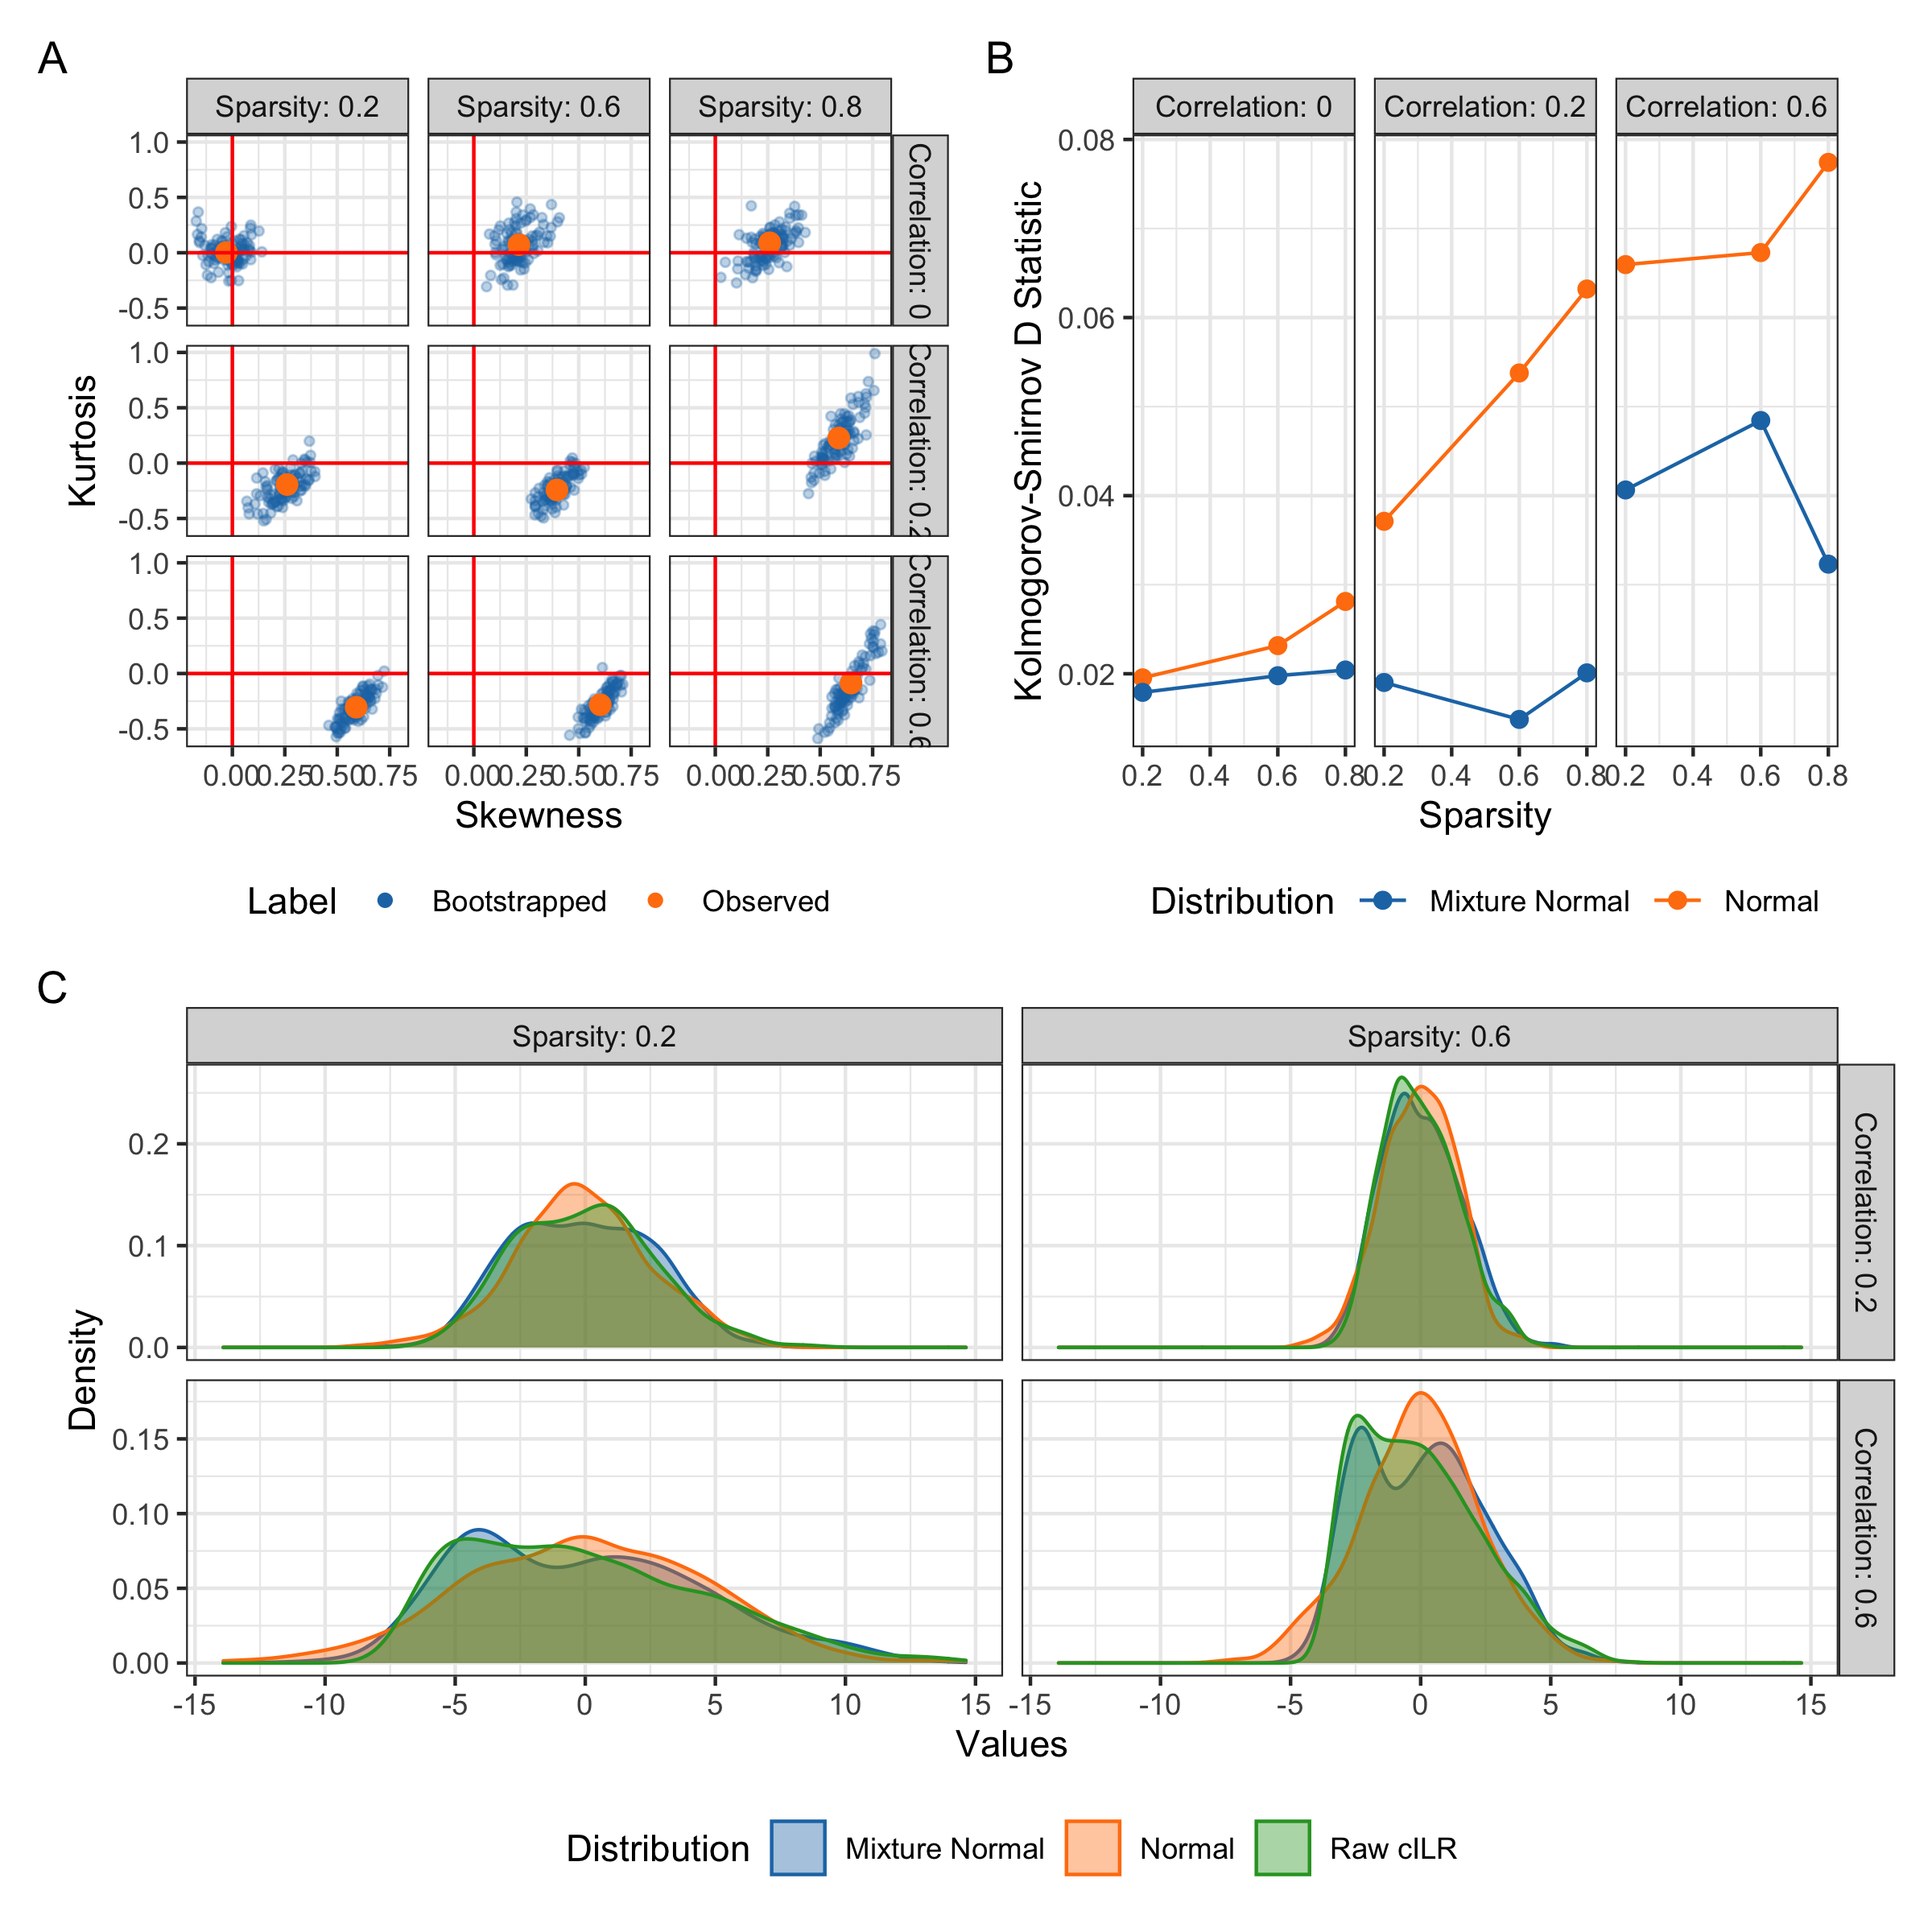
\includegraphics[width=\linewidth]{figures/kurtosis_skewness_gof.png}
    \caption{Properties of the null distribution of cILR in different simulation scenarios under the global null. Panel \textbf{(B)} presents kurtosis and skewness of cILR scores while panel \textbf{(A)} presents the goodness of fit (as Kolmogorov-Smirnov D statistic) for mixture normal and normal distributions. Panel \textbf{(C)} is a density plot of the shape of the null distribution. Results indicated the necessity of estimating an empirical null and demonstrating that the mixture distribution was the better fit compared to the basic normal.}
    \label{fig:kurt_gof}
\end{figure}

Additionally, the degree of kurtosis and skewness also suggests that the normal distribution itself might not be a good approximation of the null. To address this issue, we also evaluated a mixture distribution of two normal components. Panel B of figure \ref{fig:kurt_gof} demonstrates the goodness of fit of the mixture normal and the normal distribution using Kolmogorov-Smirnov (KS) test statistic computed on fitted normal and mixture normal distribution when fitted on cILR scores in simulation scenarios under the global null. We can see that the mixture normal distribution is a better fit (lower KS scores) than the normal distribution across both sparsity and correlation settings. 

We performed our empirical null estimation by fitting our distribution of choice and computing relevant parameters on raw cILR scores on taxa-permuted data (equivalent to gene permutation in the gene expression literature). As such, the null distribution is characterized by scores computed on sets of equal size with randomly drawn taxa. However, null distribution based on taxa-permutation is sensitive to inter-taxa correlations within the set \cite{wu2012}. Since the permutation procedure does not preserve correlation structures, estimating parameters from empirical scores on permuted data will underestimate the variance inflation due to correlation. We account for this by combining the mean estimate from permuted data with the variance estimate from unpermuted data, where the inter-taxa correlation structure remains undisturbed. However, this procedure assumes that the variance of cILR is equal under both the null and alternate hypotheses. 

\subsection*{Evaluation}
\subsubsection*{Parametric Simulations}  
To address the performance of cILR for different modeling tasks, we simulated microbiome count data under the assumption that it follows a zero-inflated negative binomial distribution, which is a good fit for real microbiome relative abundance data \cite{calgaro2020}. Suppose $X_{ij}$ are observed counts for a sample $i$ and taxon $j$, then we have the following probability model
\begin{equation}
    \mathbf{X}_{ij} =
      \begin{cases}
        0 & \text{with probability $p_j$}\\
        \mathbf{NB}(\mu_j, \phi_j) & \text{with probability $1 - p_j$}\\
      \end{cases}       
\end{equation}

where $\mu_j$ and $\phi_j$ are mean and dispersion parameters, respectively. To incorporate a flexible correlation structure into our simulation model, we utilized the NorTA (Normal to Anything) method \cite{cario1997}. Given an $n$ by $p$ matrix of values $\mathbf{U}$ sampled from multivariate normal distribution with correlation matrix $\mathbf{\rho}$, we can generate target microbiome count vector $\mathbf{X_{.j}}$ for taxa $j$ following the marginal distribution $\mathbf{NB}$ characterized by the negative binomial cumulative distribution function $\mathbb{F_{\mathbf{NB}}}$:
\begin{equation}
    \mathbf{X}_{.j} = \mathbb{F_{\mathbf{NB}}}^{-1}(\Phi_{U_i})
\end{equation}
In this instance, for each taxon $j$, we set elements in $\mathbf{U}_{.j}$ to be zero with probability $p_j$ and applied $\mathbf{NB}^{-1}(\mu_j, \phi_j)$ on non-zero elements to generate our final count matrix $\mathbf{X}$. To ensure that our simulations match closely to real data, we fitted negative binomial distribution using a maximum likelihood approach (with the \emph{fitdistrplus} package in R \cite{delignette-muller2015}) to non-zero counts for each taxon from 16S rRNA profiling of stool samples from the Human Microbiome Project (HMP). We take the median values of the estimated mean and dispersion parameters as the baseline of our simulations. For simplicity, we assumed that inter-taxa correlation follows an exchangeable structure

\noindent \textbf{Single Sample Enrichment}: To assess type I error rate and power for enrichment significance testing at the sample level, we simulated data based on the schema above, and assessed enrichment for one focal set. Type I error was obtained under the global null as the number of samples where the null hypothesis was rejected at $\alpha = 0.05$ over the total number of samples (which represents the total number of hypotheses tested). Power was obtained using the same formulation as type I error rate but under the global alternate. We treated type I error and power as estimates of binomial proportions and utilized the Agresti-Couli \cite{agresti1998} formulation to calculate 95\% confidence intervals. Across both analyses, we varied sparsity levels ($p = 0.2, 0.4, 0.6$) and inter-taxa correlation within the set ($\rho = 0, 0.2, 0.5$). For type I error analysis, we also varied the size of the set (50, 100, 150). For power analyses, set size was kept constant at 100 but different effect sizes (fold change of 1.5, 2, and 3). All sample sizes were set at 10,000. 

For classifiability, we evaluated the scores against the true labels per sample (indicating the sample has a set with inflated counts) using the area under the receiving operator curve (AUROC/AUC). This is a strategy used in Frost et al. \cite{frost2020a} which evaluates the informativeness of scores by assessing the relative ranking of samples (i.e. whether samples with inflated counts are highly ranked using estimated scores).  DeLong 95\% confidence intervals for AUC \cite{delong1988} were obtained for each estimate. Simulation settings for classification performance were identical to power analyses as detailed in the previous paragraph. 

\noindent \textbf{Differential Abundance Analysis}: To assess type I error rate and power for differential abundance testing task, we simulated data based on the schema above, and assessed differential abundance of 50 sets with 100 taxa per set across 20 replicates per simulation condition. Type I error is calculated as the number of differentially abundant sets over the total number of sets for each simulation under the global null. Power is defined similarly, but instead under the global alternate hypothesis. Estimates and confidence intervals for type I error and power are calculated as cross-replicate mean and standard error. A set is differentially abundant when all taxa within a set are differentially abundant with the same effect size. Across both analyses, we varied sparsity levels ($p = 0.2, 0.4, 0.6$), and inter-taxa correlation within the set ($\rho = 0, 0.2, 0.5$). Half of the sets are differentially abundant across case/control status with varying effect sizes (fold change of 1.5, 2, and 3). Due to the compositional nature of microbiome data, simple inflation of raw counts would cause an artificial decrease in the abundance of the remaining un-inflated sets. As such, we applied a compensation procedure as described in Hawinkel et al. \cite{hawinkel2019} to ensure the validity of simulation results. All sample sizes were set at 2,000.    

\noindent \textbf{Prediction}: To assess the predictability, we generated predictors based on the simulation schema presented above and evaluated prediction for both binary and continuous outcomes using a standard random forest model \cite{breiman2001}. For binary outcomes, we use AUC similar to the classification analyses above. For continuous outcomes, we used root mean squared error (RMSE). All predictive model fitting was performed using \emph{tidymodels} \cite{kuhn2020} suite of packages. Across both learning tasks, we varied sparsity ($p = 0.2, 0.4, 0.6$), and inter-taxa correlation ($\rho = 0, 0.2, 0.5$). Continuous outcomes $Y_{cont}$ were generated as linear combinations of taxa counts.  
\begin{equation}
    Y_{cont} = f(\mathbf{X}) + \mathbf{\epsilon}
\end{equation}
where $\mathbf{\epsilon} \sim N(0, \sigma_{\epsilon}^2)$ and $f(\mathbf{X}) = \beta_0 + \mathbf{X}\mathbf{\beta}$. For each simulation, we set $\beta_0$ to be $\frac{6}{\sqrt{10}}$ similar to \cite{xiao2018}. The degree of model saturation (the number of non zero $\mathbf{\beta}$ values) were varied between 0.1 and 0.5, and signal to noise ratio (SNR = $\frac{\sigma(f(\mathbf{X}))}{\sigma_{\epsilon}}$) was varied between 1.5, 2, and 3. 

For binary outcomes, we generate $Y_{binary}$ as Bernoulli draws with probability $p_{binary}$, where 
\begin{equation}
    p_{binary} = \frac{1}{1 + \exp(f(\mathbf{X}) + \mathbf{\epsilon})}
\end{equation}
To ensure a balance of classes, we applied the strategy described in Dong et al. \cite{dong2020} where the associated $\beta$ values are evenly split between positive and negative associations. All data sets generated from prediction tasks have 2,000 samples with 5,000 taxa over 50 sets with a size of 100 taxa per set.  

\subsubsection*{Real Datasets}

In addition to simulation analyses, we also evaluated our method using real data sets based on both 16S rRNA gene sequencing and whole-genome sequencing. All data sets are obtained from either the \emph{curatedMetagenomicData} \cite{pasolli2017} and \emph{HMP16SData} \cite{schiffer2019} R packages (2020-10-02 snapshot), or downloaded from the Qiita platform \cite{gonzalez2018}.  

\noindent \textbf{Single Sample Enrichment}: To assess the false discovery rate and true discovery rate of cILR in sample-level enrichment testing, we utilized the 16S rRNA gene sequencing of the oral microbiome at the gingival subsite from the Human Microbiome Project \cite{consortium2012, proctor2019}. We utilized this data set following the approach outlined in Calagaro et al. \cite{calgaro2020}. This data set is special because it is approximately labeled, where aerobic microbes are enriched in the supragingival subsite where the biofilm is exposed to the open air, while conversely anaerobic microbes thrive in the subgingival site \cite{thurnheer2016}. Here, we assessed the enrichment of aerobic microbes across all samples, we considered the false discovery rate as the number of samples from the subgingival site with significant enrichment, and the true positive rate as the number of supragingival samples with significant enrichment. Microbial tropism annotation at the genus level was from Beghini et al. \cite{beghini2019} and was downloaded directly from the GitHub repository associated with Calagaro et al. \cite{matteocalgaro2020}. 

\noindent \textbf{Differential Abundance Analsysis}: To assess type I error using cILR scores in differential abundance analysis, we utilized the 16S rRNA gene sequencing of stool samples from the Human Microbiome Project \cite{consortium2012, proctor2019}. Here, we randomly assign samples a label of case or control, and repeated this process 500 times, assessing all candidate methods at each iteration. Type I error is then the number of taxa identified as differentially abundant across all tested taxa. For the true positive rate, we used the same gingival data set as described above. However, instead of testing for aerobic microbes as a group, the true positive rate is the number of aerobic/anaerobic genera identified as differentially abundant across all aerobic or anaerobic genera. 

\noindent \textbf{Disease Prediction}: To assess predictive power, we utilized the whole genome sequencing of stool samples of inflammatory bowel disease (IBD) patients from the MetaHIT consortium \cite{nielsen2014}. This data set contains 396 samples from a cohort of European adults, where 195 adults were classified as having IBD (which includes patients diagnosed with either ulcerative colitis or Crohn's disease). Additionally, we also utilized a similar data set from Gevers et al. \cite{gevers2014} which also profiles the gut microbiome of IBD patients and controls but using 16S rRNA gene sequencing. This data set contains 16S rRNA gene sequencing samples from a cohort of pediatric patients (ages $<$ 17) from the RISK cohort enrolled in the United States and Canada. Of the 671 samples obtained, 500 samples belong to patients with IBD. 

\subsubsection*{Comparison Methods}

\noindent \textbf{Single sample enrichment}: For type I error and power analyses, we compared the cILR method with a naive Wilcoxon rank sum test. We added a pseudocount of 1 to all zero entry values. This is a non-parametric difference in means test, where we compared the abundance of taxa of a pre-defined set and its complement within a single sample. For classification performance, we compared cILR methods against GSVA \cite{hanzelmann2013}, ssGSEA \cite{barbie2009}, and the W-statistic from the Wilcoxon rank sum test.

\noindent \textbf{Differential Abundance}: Since cILR are sample-level enrichment scores, we performed differential abundance by using a Wilcoxon Rank Sum test and Welch's t-test across case/control status on cILR generated scores. We added a pseudocount of 1 to all zero entry values. For comparison, we chose representative state-of-the-art methods in differential abundance analysis, namely DESeq2 \cite{love2014,mcmurdie2014} and corncob \cite{martin2020}. 

\noindent \textbf{Disease Prediction}: We fit random forest on cILR scores, as well as ssGSEA \cite{hanzelmann2013} and GSVA \cite{barbie2009} similar to single sample enrichment section. We added a pseudocount of 1 to all zero entry values. Additionally, we also compared performance using enrichment scores against a standard analysis plan where the centered log-ratio transformation (CLR) was applied to count-aggregated sets as inputs to a machine learning model.  

\section*{Results}
In this section, we present the performance of our proposed method for three applicable microbiome analysis tasks: sample level enrichment, differential abundance, and disease prediction. We obtained these results from both parametric simulations and examples from real data.  

\subsection*{Enrichment testing at the sample level}
cILR provides significance testing for enrichment at the sample level using the null distribution estimation procedure described in \nameref{Methods}. Here, we present empirical results for this application of cILR assessing type I error, power, and classification capacity. 

Panel A and B in figure \ref{fig:ss_hypo} demonstrate type I error and power respectively across different simulation conditions. We benchmarked the results of the cILR method against a naive Wilcoxon rank sum test performed at the sample level, comparing the mean count difference between taxa in the set its complement. All methods demonstrate good type I error control at $\alpha = 0.05$ under zero correlation across all simulation conditions. However, under both medium ($\rho = 0.2$) and high ($\rho = 0.5$) correlation settings, both the Wilcoxon test and unadjusted cILR variants show high levels of inflated type I error, where Wilcoxon test performed the worst. On the other hand, adjusted cILR methods (under both distributions) control for type I error at the appropriate $\alpha$ level even at high correlations. 

\begin{figure}[H]
    \centering
    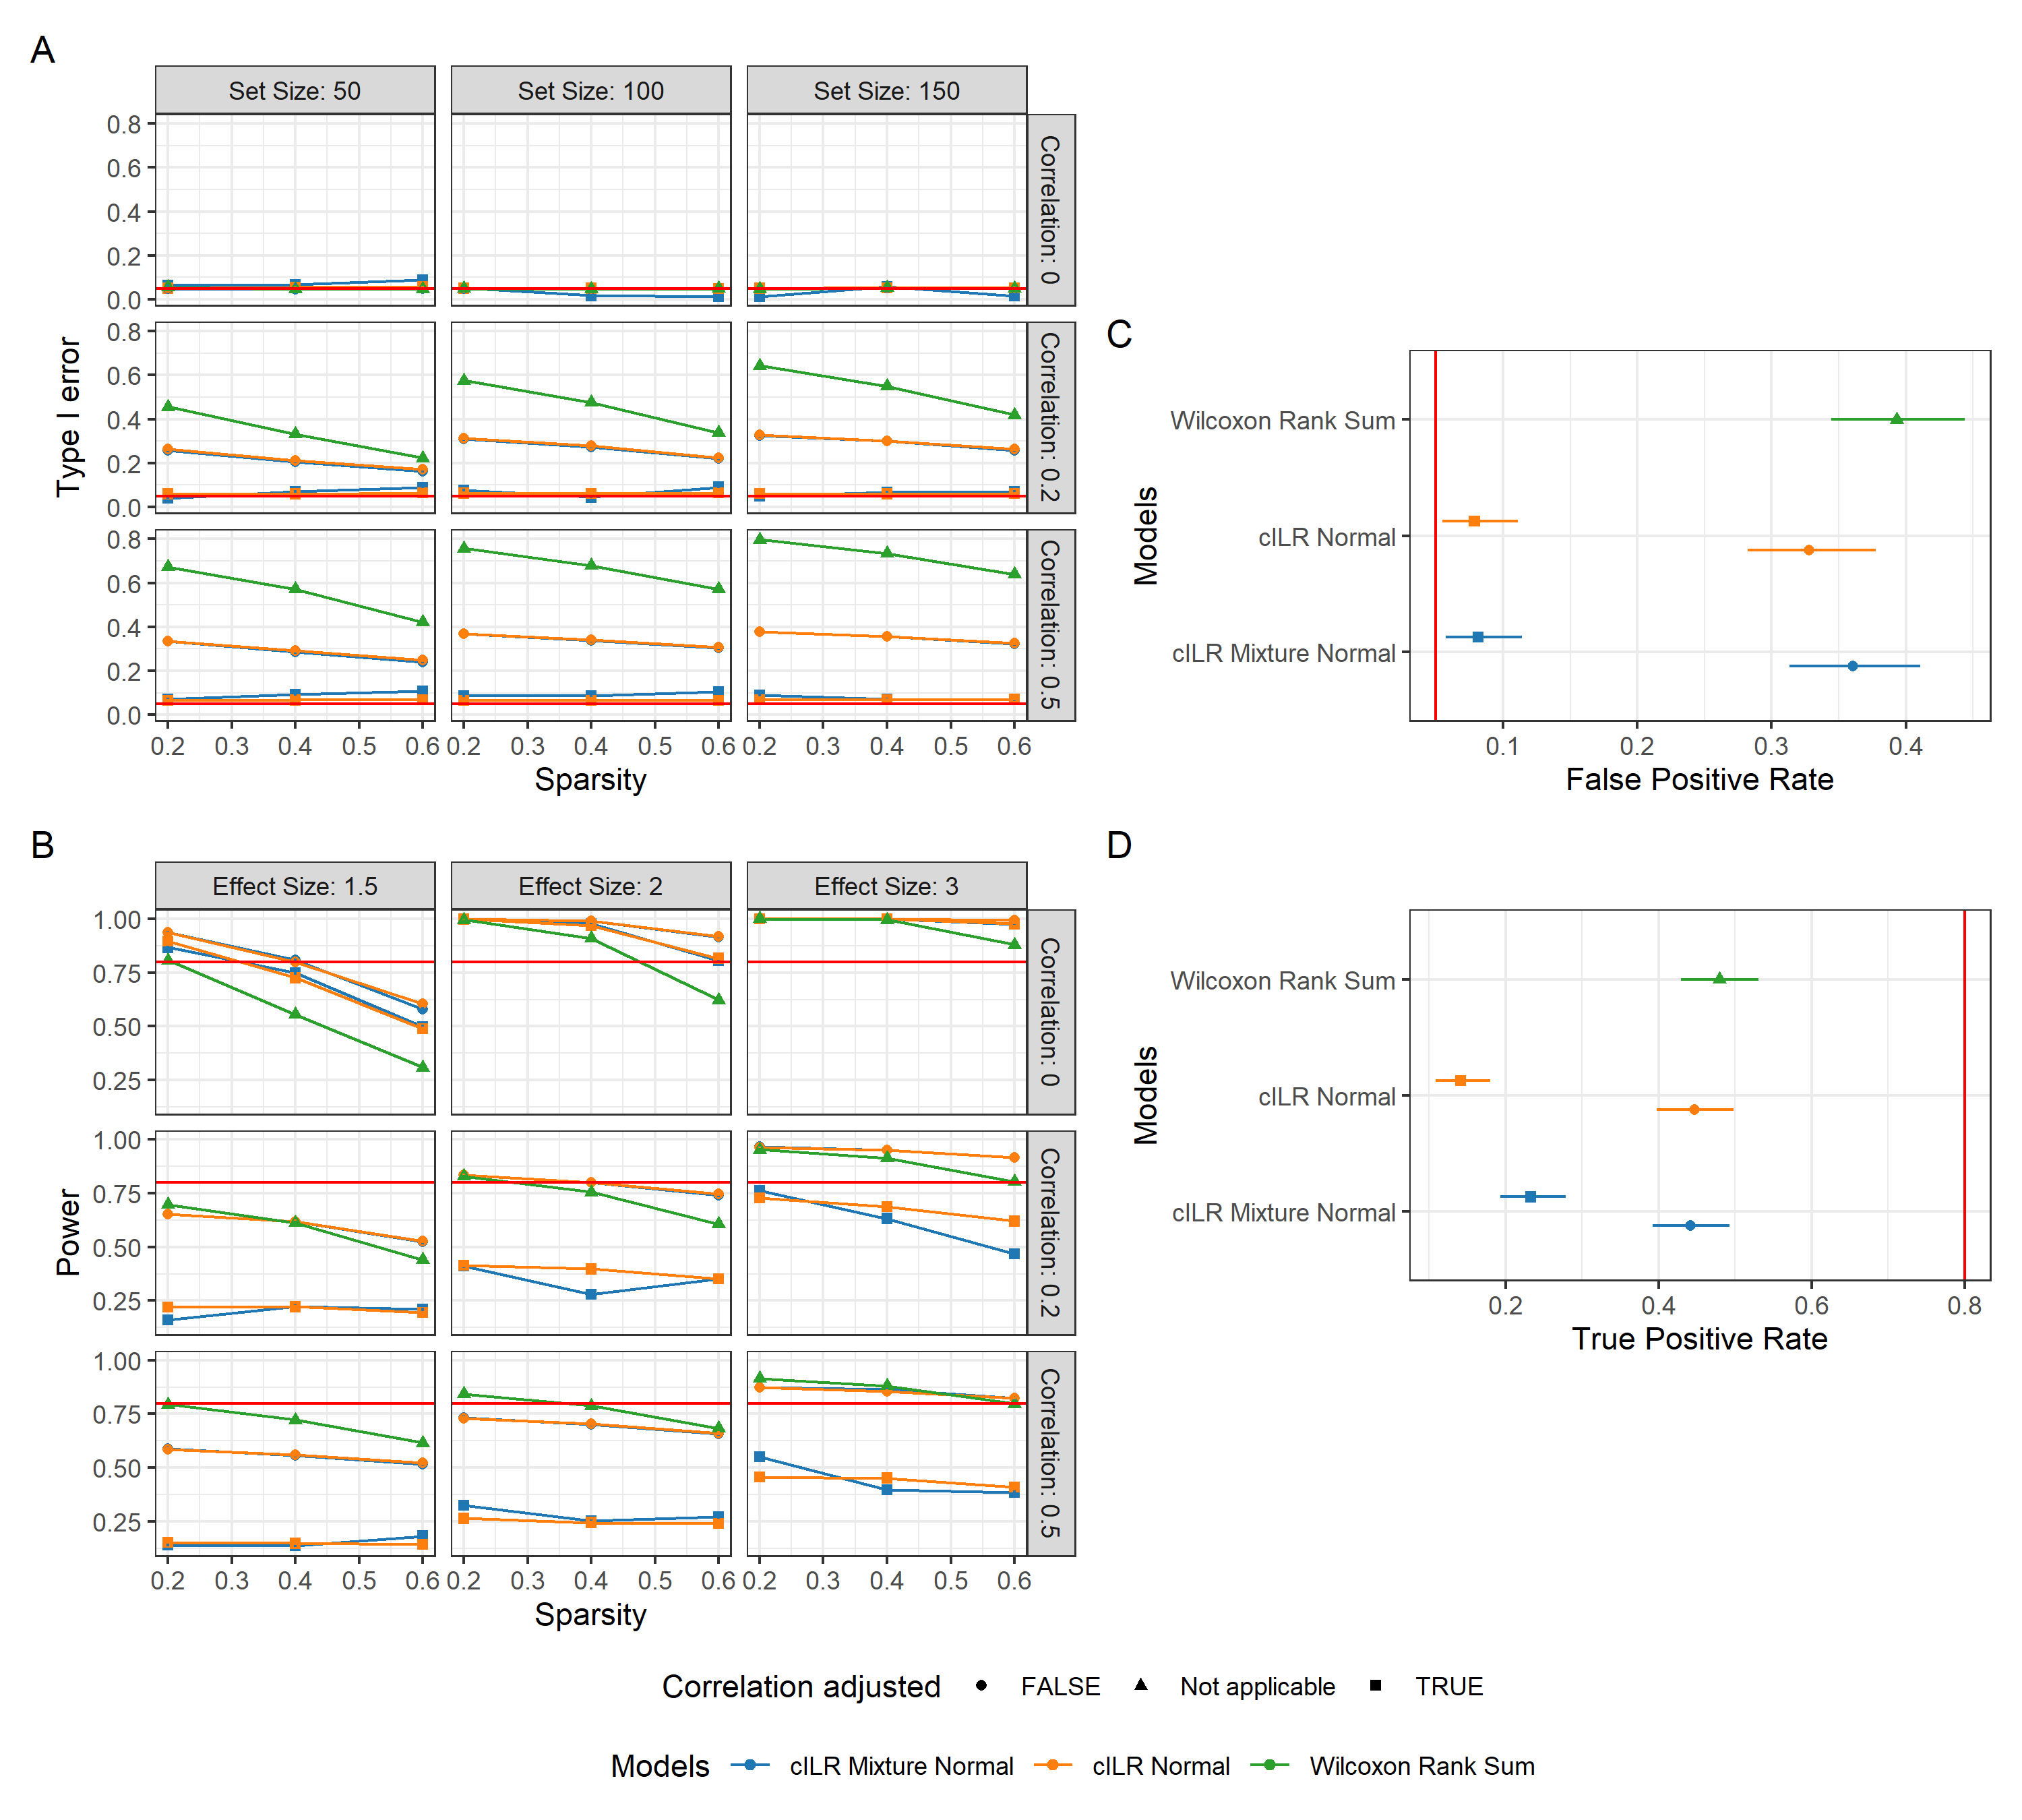
\includegraphics[width=\textwidth]{figures/sim_data_ss_hypo.png}
    \caption{Type I error rate \textbf{(A)}, and power \textbf{(B)} across different parametric simulation scenarios. Confidence bounds were obtained using Agresti-Couli \cite{agresti1998} approach. False-positive rate \textbf{(C)} and true positive rate \textbf{(D)} evaluation of similar methods on real 16S rRNA data from the oral microbiome of the gingival site. For \textbf{(A)} and \textbf{(B)}, enrichment of a specified set was tested at the sample level using cILR and the Wilcoxon rank sum test at $\alpha$ of 0.05. For \textbf{(C)} and \textbf{(D)}, the set of aerobic microbes was tested for enrichment in all samples and was identified as correctly enriched if a significant $p$-value was obtained in supragingival samples. Adjusted cILR demonstrated control of type I error at the appropriate $\alpha$ level while remaining methods (not included in subsequent power analyses) showed an inflated type I error rate. However, this resulted in lower power for adjusted cILR methods.}
    \label{fig:ss_hypo}
\end{figure}

However, the trade-off for good type I error control is demonstrably lower power, as shown in figure \ref{fig:ss_hypo}B. In situations where there is no inter-taxa correlation, cILR still outperforms the wilcoxon rank sum test, however adjusted versions of cILR did not perform as well as un-adjusted ones. However, in higher correlation scenarios, the difference in power is much more dramatic. At the highest effect size (fold change of 3) and correlation ($\rho = 0.5$), adjusted cILR was only performing at 50\% power, while unadjusted cILR and wilcoxon rank sum test were able to reach 80\%. These results indicate that both sparsity and inter-taxa correlation impacts power, with correlation having a much more dramatic impact especially for adjusted versions of cILR. Most importantly, cILR demonstrate higher power in all scenarios where type I error is properly controlled.    

These observations were replicated when assessed on the semi-labeled gingival data set from the Human Microbiome Project as described in \nameref{Methods}. Here, we tested the enrichment of aerobic microbes for each sample using approaches similar to our parametric simulations. As expected in Figure \ref{fig:ss_hypo}C, the proportion of falsely rejected hypotheses was high in the naive Wilcoxon test and unadjusted cILR methods. Conversely, adjusted cILR controls for false positives adequately at the correct $\alpha$ level of 0.05. Power analysis (Figure \ref{fig:ss_hypo}D) showed similar patterns, where unadjusted cILR methods and the Wilcoxon test have a higher proportion of null hypotheses correctly rejected, however, these results are not useful to a practitioner as the number of falsely rejected hypotheses are also equally high.  

To further assess the utility of cILR in classifying samples with enriched sets, we generated AUC scores for different cILR scores using true labels of whether a sample has an inflated set. This analysis, therefore, assessed the relative ranking of samples using cILR scores whereby high scores should correspond to samples that are known to be inflated. Figure \ref{fig:ss_auc} presents this result. We compared different variants of cILR against competing methods in the gene set testing space (GSVA \cite{hanzelmann2013} and ssGSEA \cite{barbie2009}), as well as the $U$ test statistic from the Wilcoxon rank sum test. Across both simulations (Figure \ref{fig:ss_auc}A) and real-data applications (Figure \ref{fig:ss_auc}B), cILR scores perform marginally better especially in low effect size situations but did not stand out in most other scenarios. In simulation studies, classification performance was good (around AUC of 0.8) even at high correlation settings, only requiring medium effect sizes (fold change of 2). Notably, the W-statistic provided the least information for classifying samples with inflated taxa.

\begin{figure}[H]
    \centering
    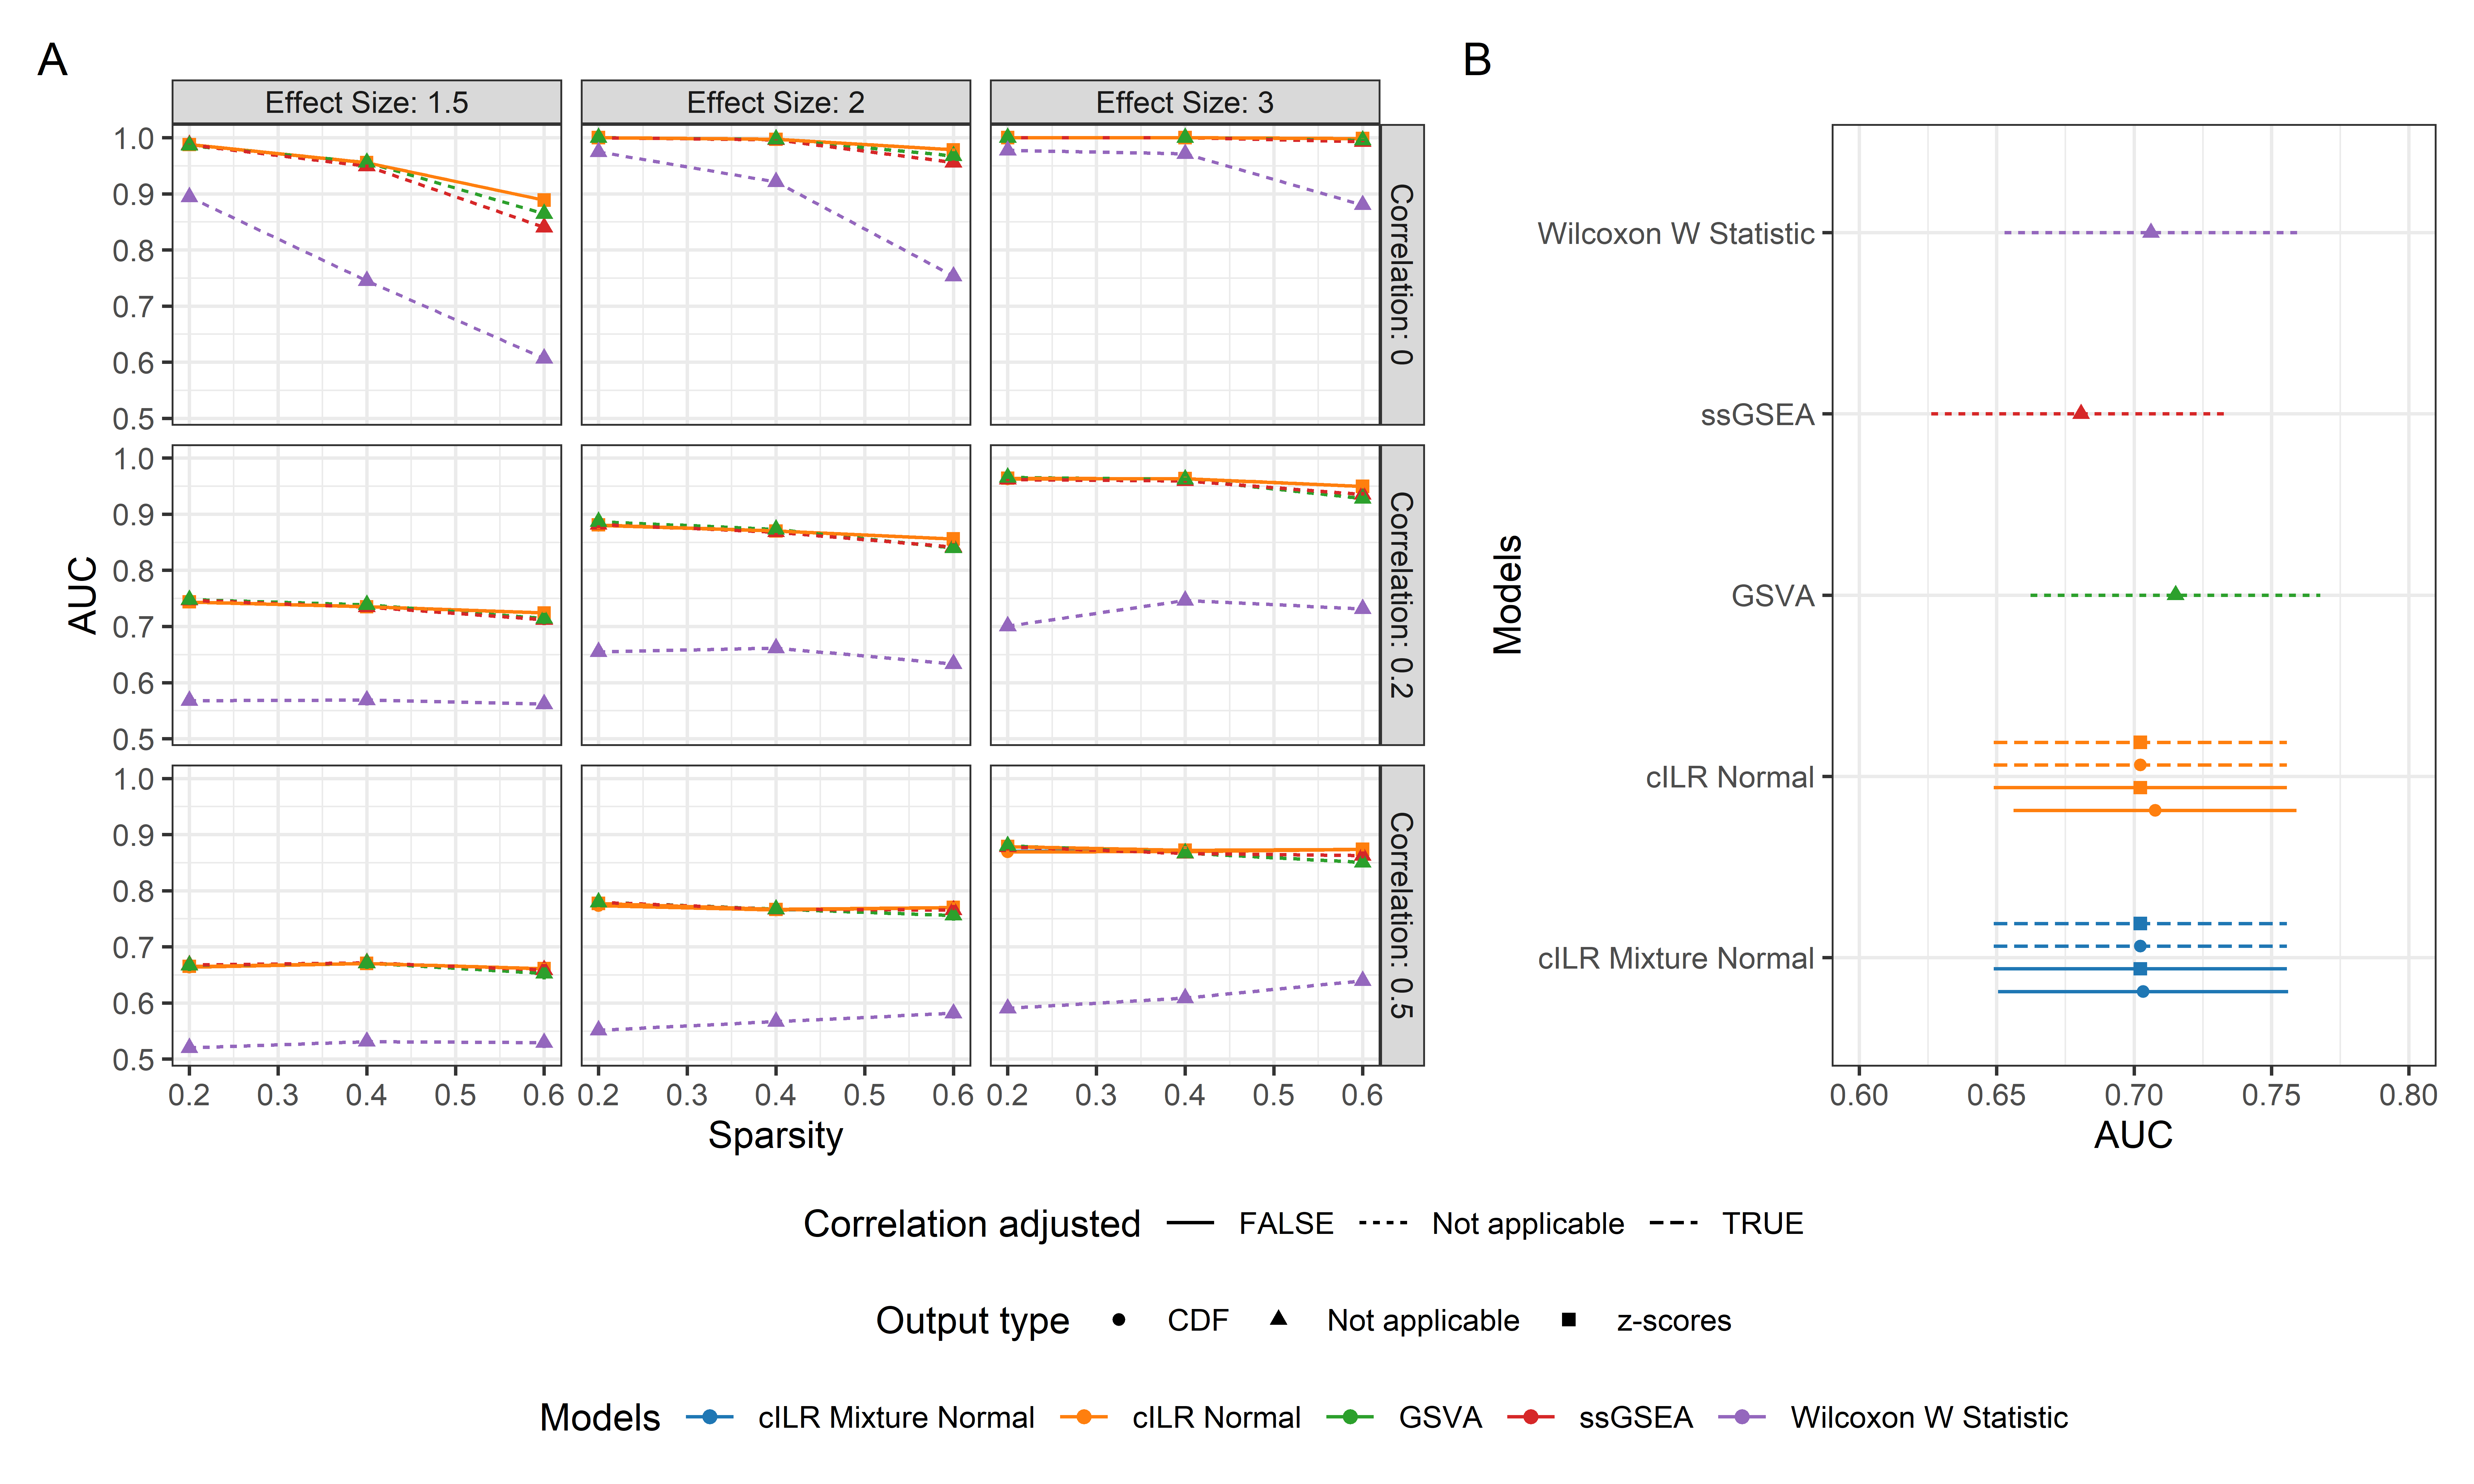
\includegraphics[width = \textwidth]{figures/sim_data_ss_auc.png}
    \caption{Classification performance via AUC of cILR, ssGSEA, GSVA, and Wilcoxon $U$ statistic on simulated data \textbf{(A)} the gingival data set from the Human Microbiome Project  \textbf{(B)} as detailed in \nameref{Methods}. Performance scores measure whether scores can highly rank samples that are known to have inflated abundance. In the gingival data set presented in panel \textbf{(B)}, samples from the supragingival site are assumed to have an inflated abundance of aerobic microbes. Error bars are the 95\% DeLong confidence intervals for AUC \cite{delong1988}} 
    \label{fig:ss_auc}
\end{figure}

\subsection*{Differential abundance analysis}
Here we assessed the ability to use cILR with a standard difference of means statistical test (such as Welch's t-test or a Wilcoxon rank sum test) to perform differential abundance analysis. We compared the performance of cILR related methods to two commonly used approaches in the microbiome literature: DESeq2 \cite{love2014} and corncob \cite{martin2020}.   

\subsection*{Disease Prediction} 
We can conceive of cILR as a feature engineering step before model fitting and prediction. Here we assessed the predictive performance of a standard machine learning model (random forest \cite{breiman2001}) using cILR scores compared to scores generated by other single sample enrichment methods in the gene set testing literature (ssGSEA \cite{barbie2009} and GSVA \cite{hanzelmann2013}). Additionally, we also compared our results with the use of the centered log-ratio (CLR) transformation on taxa sets aggregated via count summations.    

Figure \ref{fig:sim_pred_auc} and \ref{fig:sim_pred_rsq} showed results from simulation studies as detailed in the \nameref{Methods} section under both classification and regression tasks. As expected, performance across all assessed methods increased with a higher signal-to-noise ratio, however, they remained consistent across different levels of model saturation and inter-taxa correlation. Importantly, cILR methods outperformed both GSVA and ssGSEA, where the difference in AUC increases as a function of sparsity. Conversely, cILR scores did not perform as well as the traditional CLR approach, however, the performance gap decreased at higher sparsity levels. Similar patterns were observed for regression results (Figure \ref{fig:sim_pred_rsq}). Most interestingly, regression performance, in general, decreased at higher saturation levels (proportion of sets associated with the outcome). cILR remained more performant than both ssGSEA and GSVA, but was still less than the standard CLR, especially at higher signal-to-noise ratios. Similarly, cILR still performed much better in higher sparsity situations, where the results were almost identical to the CLR approach, especially in high saturation scenarios.     

\begin{figure}[H]
    \centering
    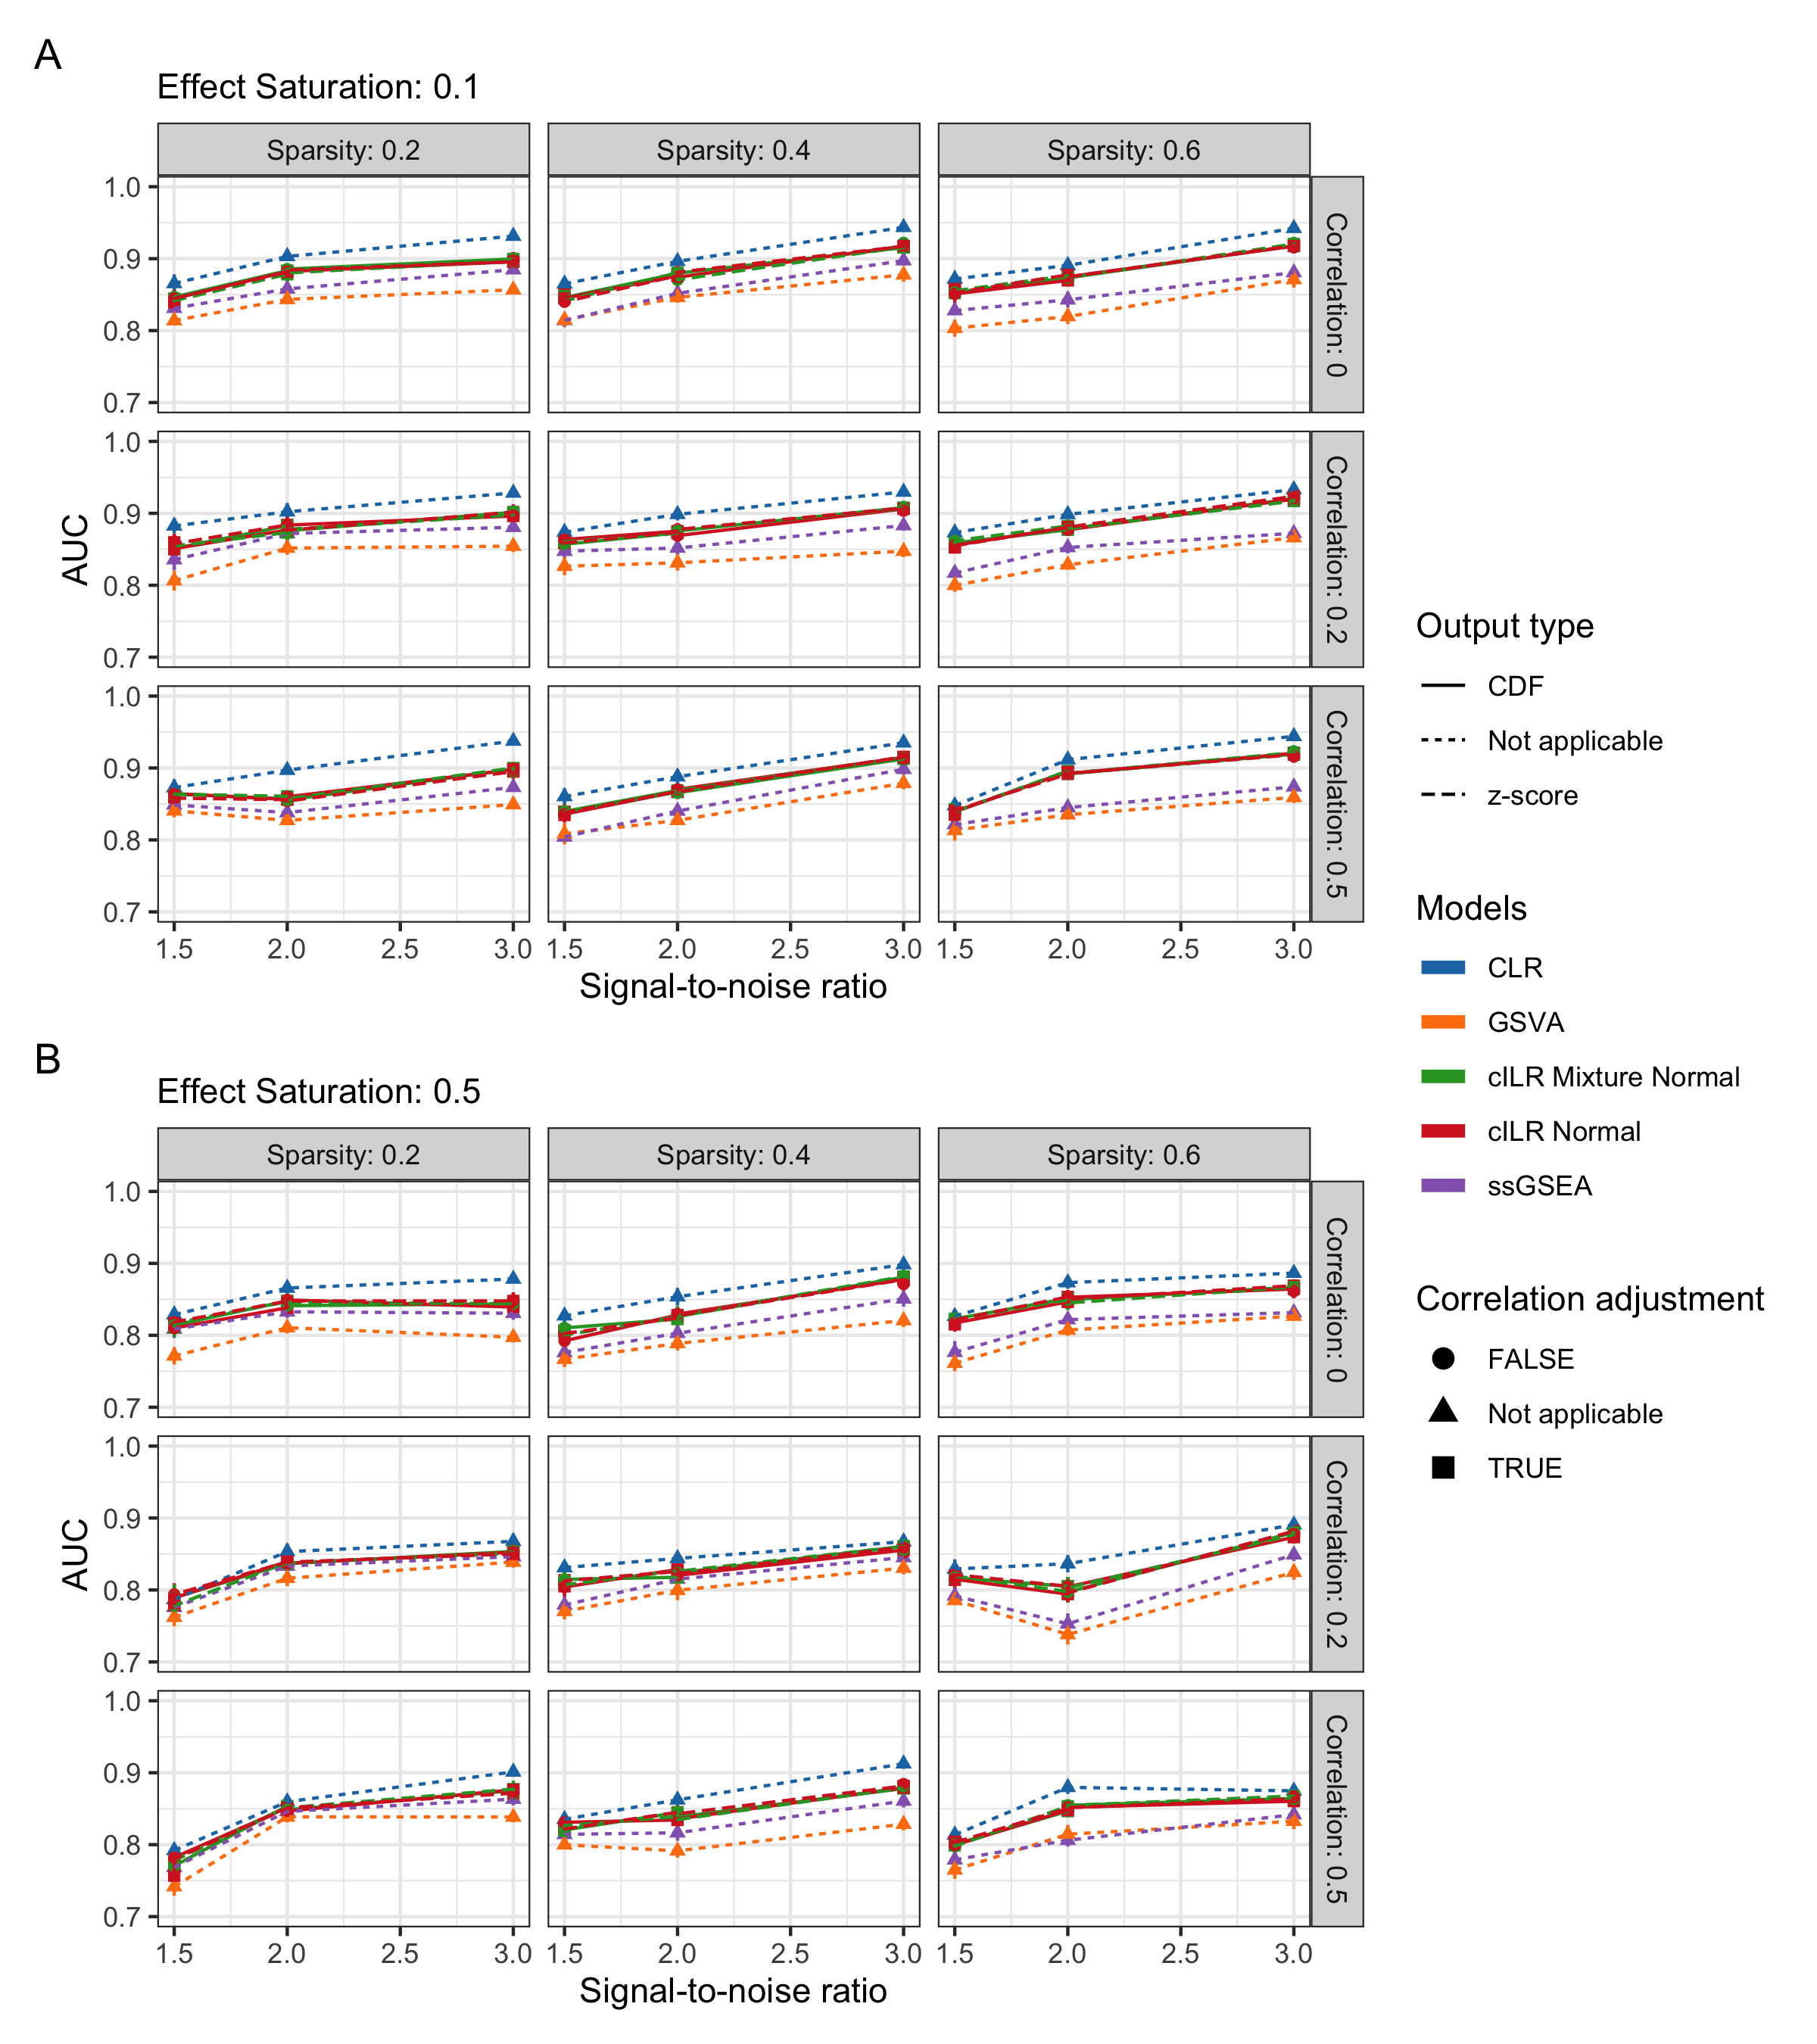
\includegraphics[width=\textwidth]{figures/sim_pred_auc.png}
    \caption{AUC scores of a random forest model for a binary outcome trained on cILR, ssGSEA, GSVA generated scores as well as on standard CLR transformed data evaluated on simulated data across sparsity levels, correlation, and signal-to-noise ratio. Panel \textbf{(A)} and \textbf{(B)} represent results across different levels of model saturation (proportion of sets associated with the outcome). cILR approaches outperformed GSVA and ssGSEA but not standard CLR.}
    \label{fig:sim_pred_auc}
\end{figure}


\begin{figure}[H]
    \centering
    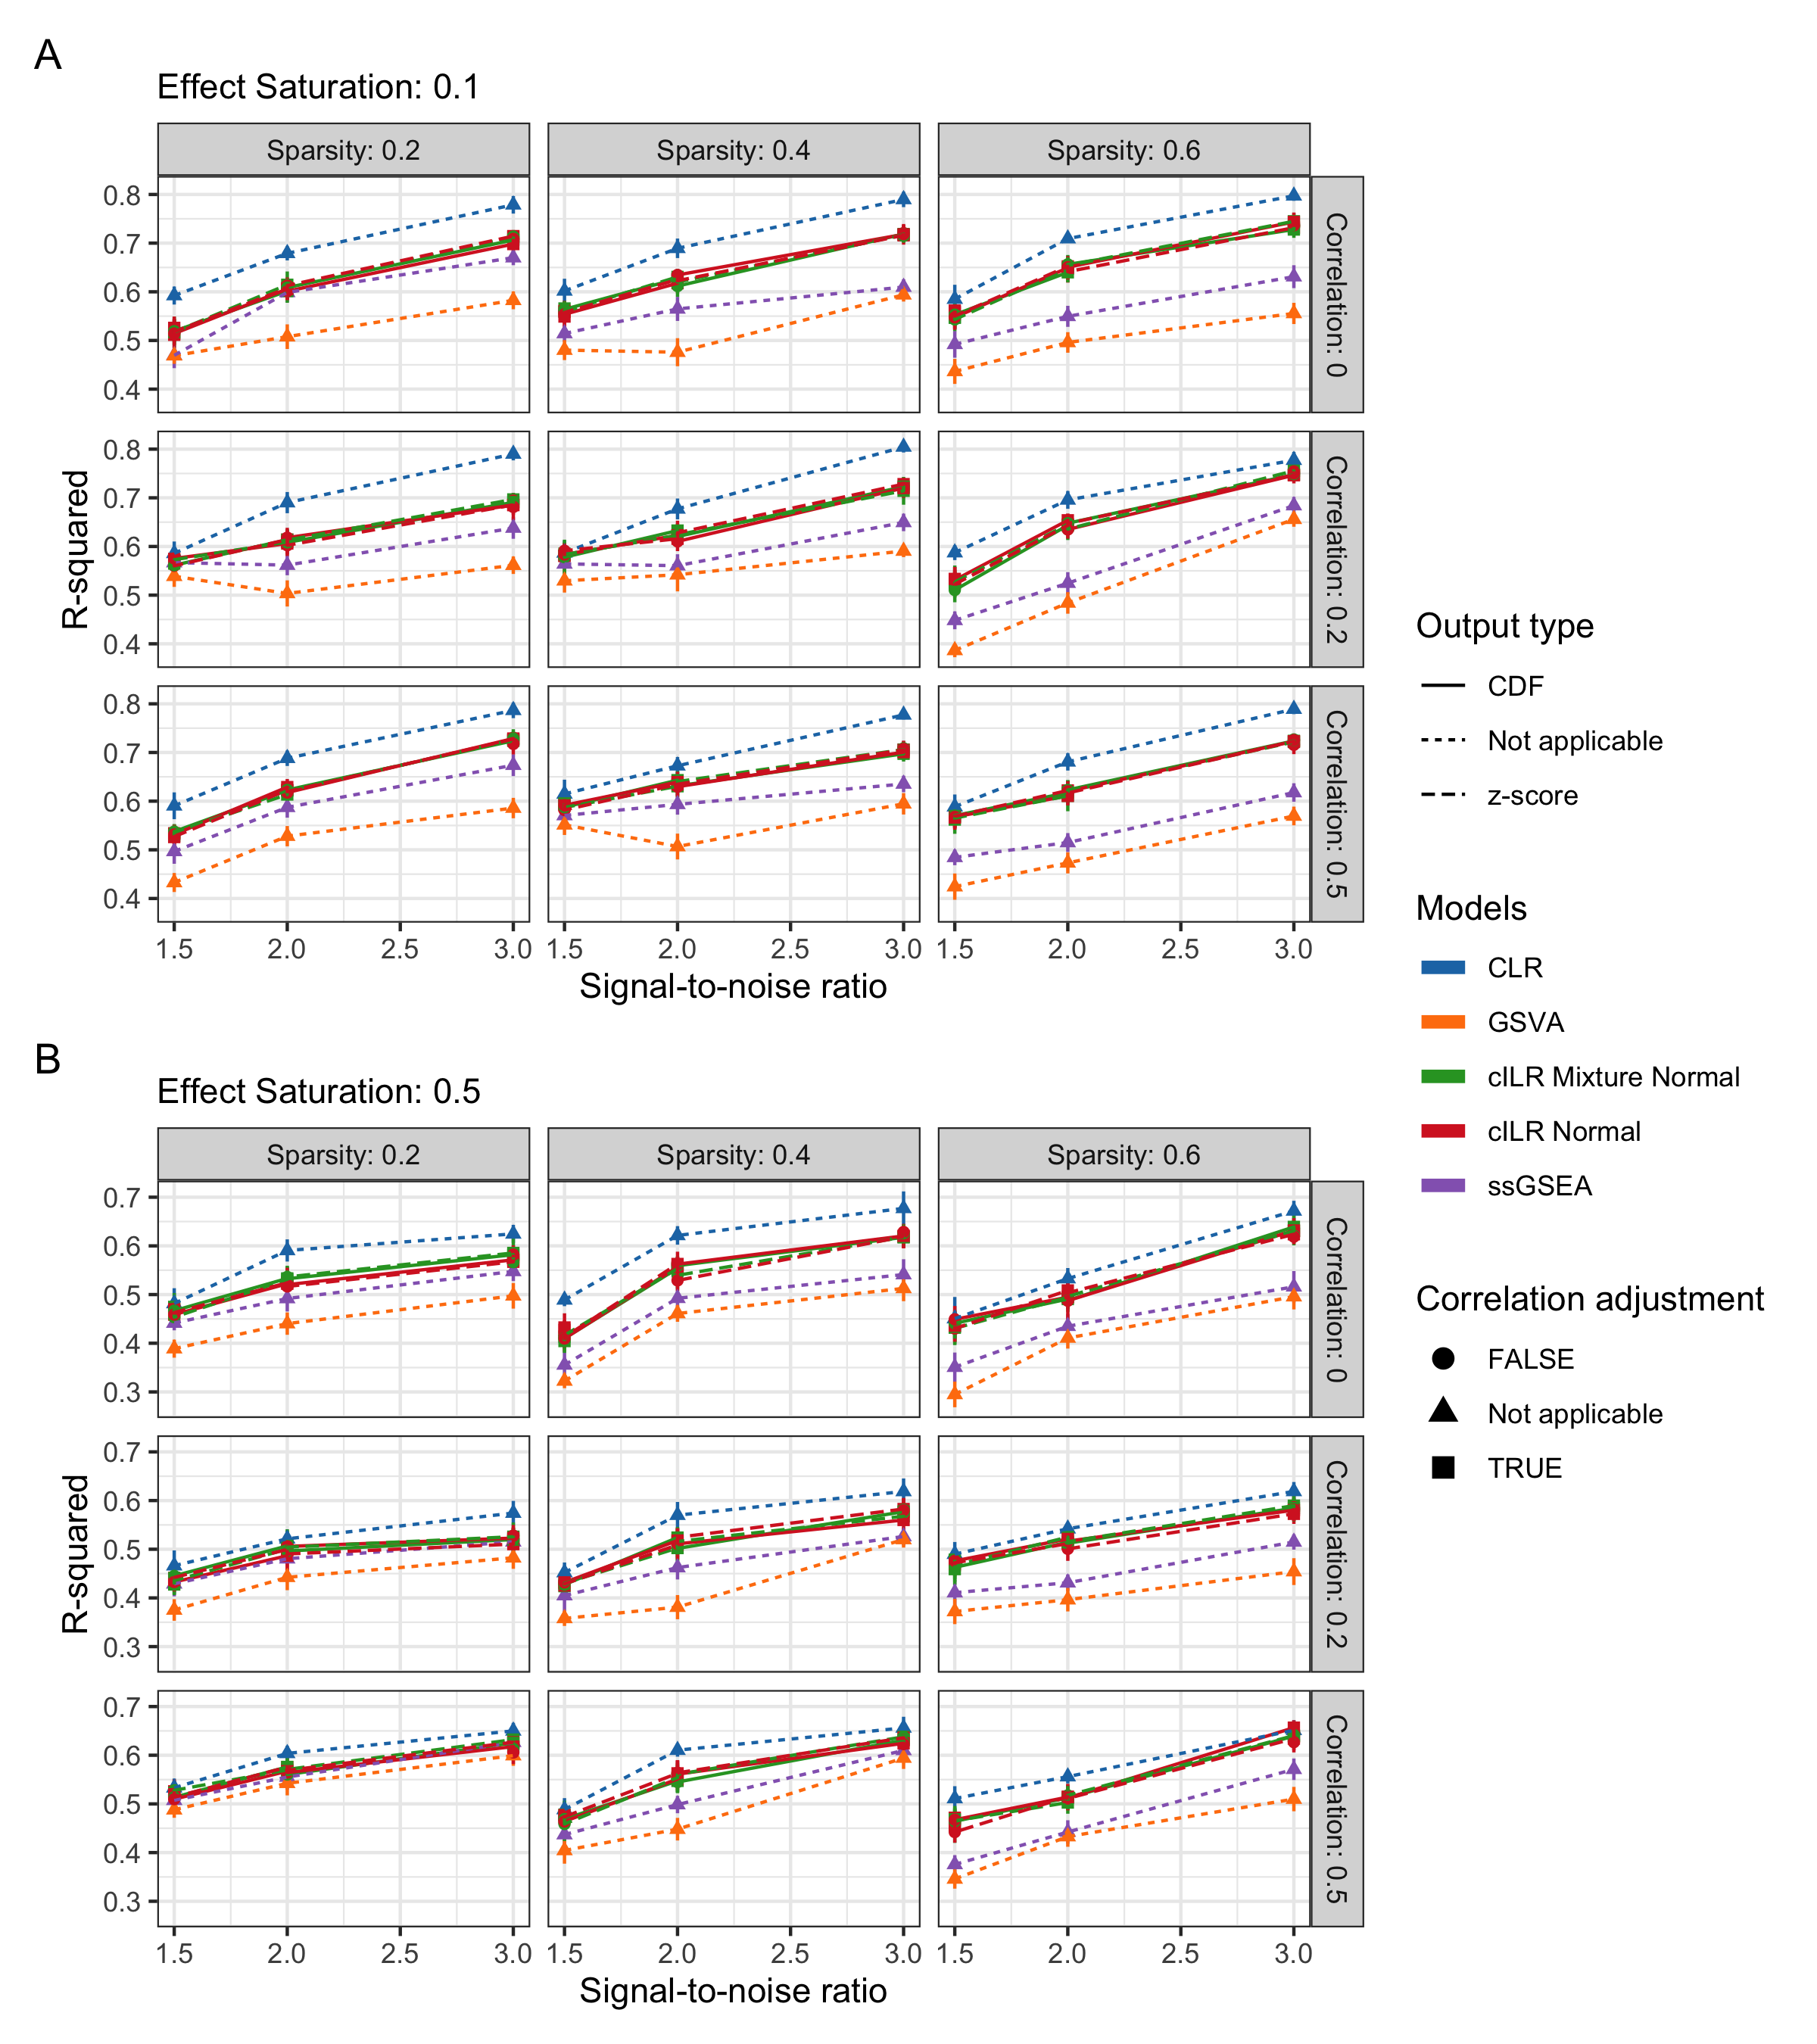
\includegraphics[width=\textwidth]{figures/sim_pred_rsq.png}
    \caption{Predictive R-squared of a random forest model for a continuous outcome trained on cILR, ssGSEA, GSVA generated scores as well as on standard CLR transformed data evaluated on simulated data across sparsity levels, correlation, and signal-to-noise ratio. Panel \textbf{(A)} and \textbf{(B)} represent results across different levels of model saturation (proportion of sets associated with the outcome). cILR approaches outperformed GSVA and ssGSEA but not standard CLR.}
    \label{fig:sim_pred_rsq}
\end{figure}

In addition to parametric simulations, we also demonstrated predictive performance using real data sets in Figure \ref{fig:pred_data}. The learning task across both data sets is to classify patients who are diagnosed with inflammatory bowel disease (includes both Crohn's disease and ulcerative colitis) and healthy controls. The Gevers et al. \cite{gevers2014} data set is a 16S rRNA sequencing data set while the Nielsen et al. \cite{nielsen2014} is a whole-genome shotgun sequencing data set. Similar to simulation experiments, across both data sets cILR methods provide much better performance than either GSVA or ssGSEA. Interestingly, the standard CLR approach only outperformed cILR in the 16S rRNA data set but was marginally worse in the WGS data set. Additionally, we observed that using the normal distribution for cILR generates better predictive performance compared to the other variants.

\begin{figure}[H]
    \centering
    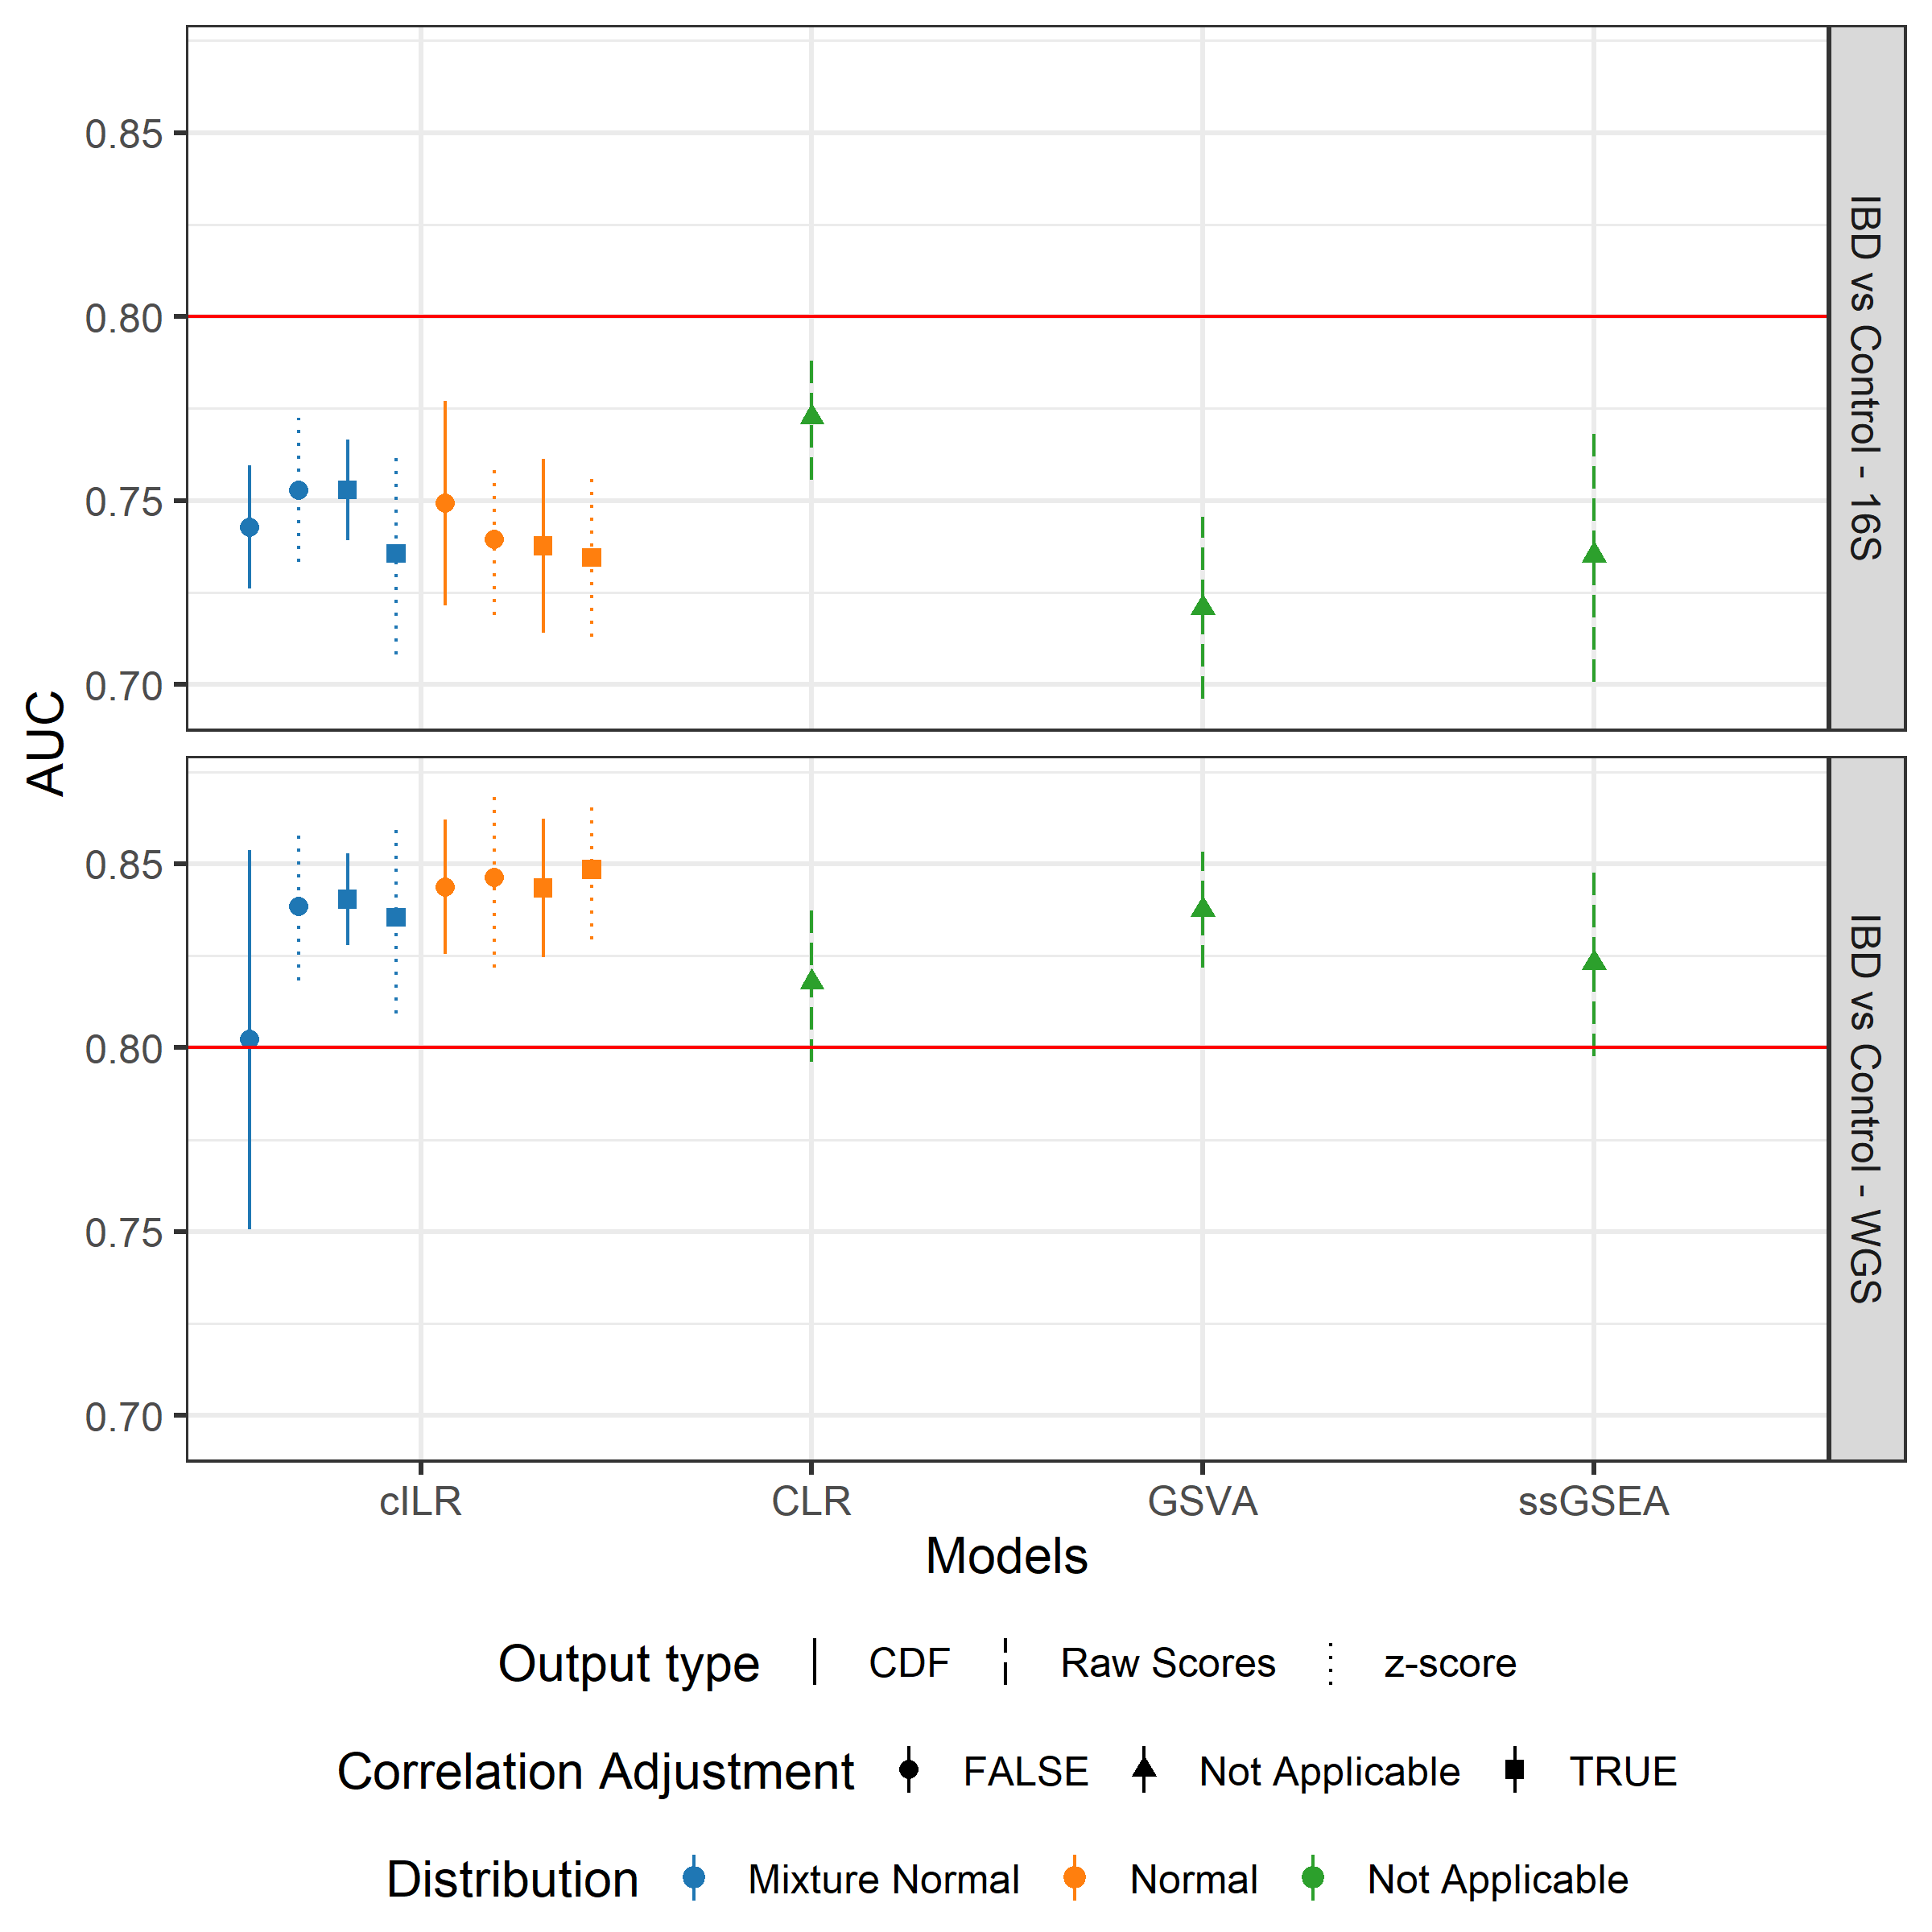
\includegraphics[scale = 0.6]{figures/data_prediction_plot.png}
    \caption{Classification performance of a standard random forest model using cILR scores compared against existing methods in gene set testing literature and the standard centered-log ratio transformation approach. The learning task involves predicting patients with inflammatory bowel disease (including Crohn's disease and ulcerative colitis) versus controls. Data sets used span both 16S rRNA sequencing (Gevers et al. \cite{gevers2014}) and whole-genome shotgun sequencing (Nielsen et al. \cite{nielsen2014}). cILR marginally outperforms GSVA and ssGSEA in both data sets, but only performs better than CLR in the WGS data set.}
    \label{fig:pred_data}
\end{figure}

These results demonstrate that cILR generated scores are informative features in disease prediction tasks. Simulation results indicate that cILR methods perform much better than either GSVA or ssGSEA, but not as well as the standard CLR approach. Interestingly, however, cILR methods were much more competitive with CLR in either WGS data sets or data sets with higher sparsity levels. 


\section*{Discussion}

\subsection*{Inference with cILR}
We can use cILR to test for enrichment of taxa-sets at the sample level. Inter-taxa correlation can result in an inflated variance of resulting test statistics \cite{wu2012}, which results in an inflated type I error if not properly controlled for. Our method addresses this issue by combining the mean estimate of scores computed on permuted data and the variance estimate of scores computed on unpermuted data, where correlation is undisrupted. As a consequence, adjusted cILR methods control very well for type I error at the appropriate $\alpha$ level (Figure \ref{fig:ss_hypo}). The conservativeness of the test persisted across different sparsity levels, as well as inter-taxa correlation. Conversely, the unadjusted cILR methods and the naive Wilcoxon rank sum test has inflated type I error even at low correlation levels ($\rho = 0.2$). However, the trade-off for proper type I error control is lower power. Simulation results showed that power is sensitive to sparsity across all correlation levels. 

However, if there is no correlation between members of a set, cILR was still able to maintain 80\% power even with low effect size (fold change of 1.5), long as the set of interest is more densely populated, such as a set of core taxa that are prevalent across all samples. Unfortunately, this relationship doesn't hold for higher correlation levels. This means that in sets where associated taxa are highly correlated, a higher fold change is required for cILR to detect enrichment. 

We also assessed cILR using different distribution forms, the normal distribution, and the mixture normal distribution. The difference in performance across the two choices was minimal, where both were able to control for type I error, but the normal distribution was slightly better when it comes to power only in certain simulation settings. This runs contrary to our distribution comparison analysis in Figure \ref{fig:kurt_gof}, where the mixture distribution was the superior fit. We hypothesized that this might be due to the difficulty in fitting mixture distributions using the expectation-maximization algorithm (EM), as the convergence rate is slow when there is a lot of overlap between the mixtures and the mixing coefficients of one of the components are low \cite{naim2012}. Furthermore, there is a lot of degeneracy of parameter values in our variance adjustment procedure for the mixture distribution(Supplemental Material). These distribution fitting problems might introduce issues where the mixture distribution might not be the best fit. As such, improvements to mixture distribution fitting might allow for better performance to be extracted.  

These results are replicated in our real data analysis, where we attempted to test for enrichment for a group of aerobic taxa among samples in the gingival site from HMP \cite{consortium2012}. Even though our labeling is not perfect, it is encouraging to see that the false discovery rate is low (approximately 0.05) when tested among a set of hypotheses where there is a mixture of true null and alternate situations. We believe that a practitioner can identify many interesting samples to follow up on by applying multiple testing adjustment procedures (such as Benjamini-Hochberg \cite{benjamini1995}) with cILR p-values and using less stringent criteria (e.g. 0.1 false discovery rate).  

In short, we demonstrated that cILR can be used to test for significance testing at the sample level. Even though there is not a lot of difference between the distribution choices, ultimately cILR controls for type I error well despite tradeoffs in power. Even then, cILR will still be able to detect enriched sets in high correlation and sparsity situations insofar as the effect size is large. Researchers can utilize cILR to test for enrichment of a certain set of taxa of interest to perform follow-up experiments or to identify the prevalence of certain sub-population of taxa (for example, oxygen preference as in our real data example). The conservativeness of the test ensures confidence in detected samples.  

\subsection*{Using cILR as inputs for downstream analyses}
Since cILR generates enrichment scores for each set at the sample level, they can be used in downstream analyses alongside standard statistical approaches. In this section we assessed the utility of cILR generated scores in two common analysis tasks in microbiome research: differential abundance testing and disease prediction.

For disease prediction, we benchmarked a basic random forest model \cite{breiman2001} to predict whether or not a patient has IBD given only their microbiome profile using cILR and relevant methods as inputs. Across both simulations and real data analyses, cILR scores perform better than alternative single sample scoring methods in the gene set testing literature (GSVA \cite{hanzelmann2013} and ssGSEA \cite{barbie2009}). This is consistent with previous analysis (Figure \ref{fig:ss_auc}), where we assessed the informativeness of cILR generated scores by using AUC to measure whether samples with high scores correspond with the true label of an inflated set. Results indicated that cILR scores are more adaptive to microbiome data sets than GSVA and ssGSEA. However, cILR scores underperform the standard approach of applying the CLR transformation to count aggregated data, except for the WGS real data analysis. Despite this, there are still benefits to using cILR scores in the context of downstream modeling beyond random forest predictive models. First, CLR transformed variables have a sum to zero constraints, making the covariance matrix is singular \cite{gloor2017}, impacting methods that rely on matrix decomposition such as principal component regression or canonical correlation analysis. Second, cILR provides an additional value of significance testing for enrichment for sample screening. Third, CLR transformed variables still involve the count summation procedure for variable aggregation, therefore comparison between sets of different sizes remains unviable.       

Despite such drawbacks, cILR methods still produce competitive performance values across both regression and classification tasks even in low signal-to-noise settings. Most interestingly, the performance gap between cILR and CLR was smaller in high sparsity settings ($p = 0.6$), which is a feature of microbiome relative abundance data \cite{li2019}. Furthermore, these predictive models consider the effect of variables jointly (and in the case of random forest, consider interactions as well), and good performance also indicated that cILR scores can also capture the joint distribution of considers sets, especially with regards to their relationship with a defined outcome such as IBD status.   

Unsurprisingly, different variants of cILR did not differ significantly in performance similar to significance testing experiments. Even though we expect Z-scores to perform better due to the added information of directionality of enrichment, using CDF values did not alter performance in both the single sample AUC evaluations (Figure \ref{fig:ss_auc}) as well as the random forest evaluations (Figure \ref{fig:sim_pred_auc}). 

In short, users can apply cILR generated enrichment scores as inputs to downstream analyses, especially predictive models and differential abundance analysis. cILR scores are informative in discriminating samples between classes even in low effect size situations. Even though cILR did not outperform a standard analysis of count aggregation followed by the CLR transformation, the additional benefits listed above would prove to be attractive in certain use cases, especially in high sparsity situations. 

\subsection*{Limitations and future directions}
There are various limitations to using cILR to generate sample-level taxonomic aggregation for microbiome data. First, significance testing at the sample level is not powered to assess inflated sets with low effect size. Practitioners can be confident in the validity of a significant result (following proper multiple testing correction) due to cILR's type I error control, but should not expect cILR to be able to identify all samples with inflated counts. Second, even though cILR is flexible and addresses the compositional nature of microbiome data, the performance of cILR might not be consistently better than competing methods. Careful evaluation of methods should be done before application to ensure that the value of cILR scores is appropriately extracted in suitable models. Third, cILR did not directly address the zero-inflatedness of microbiome data and utilizes a pseudocount to ensure log operations are valid. As such, practitioners are encouraged to choose a different pseudocount or an appropriate method of choice.   

As such, we hope to address the aforementioned issues with cILR in later projects. First, we hope to refine the distribution fitting procedure for the mixture distribution due to its superior fit and address the identifiability problem that might underlie the lack of power in our experiments. Second, we hope to incorporate some of the sophisticated model-based zero correction methods \cite{martin-fernandez2012,kaul2017a}. Third, we can account for the difference in importance of certain taxa by incorporating taxa-specific weights. Finally, we also hope to curate more interest apriori sets that are functionally informative, which would generate more interesting insight and improve interpretability compared to using taxonomic categories such as Phylum or Genus. 

\section*{Conclusion}
Gene set testing, or pathway analysis is an important tool in the analysis of high-dimensional genomic data sets. However, there has not been a lot of set-based analysis methods developed specifically for microbiome relative abundance data. In this manuscript, we introduced a new microbiome-specific method to generate set-based enrichment scores at the sample level. We demonstrated that our method can control for type I error for significance testing at the sample level, while generated scores are also valid inputs in downstream analyses, including disease prediction and differential abundance. 

\newpage
\bibliography{tax_agg}{}
\bibliographystyle{plos2015}
\end{document}